%03introduction.tex
\renewcommand\thesection{\arabic{section}}
\chapter{Management Summary}
\section{Problemstellung}
Je nach Untergrund, Bodeneigenschaften, Gel\"ande sowie Klima gedeihen in der Schweiz unterschiedliche Typen von W\"aldern. Seit einigen Jahrzehnten werden diese Typen von Experten erhoben und kartiert. Es wurden dabei verschiedene typisierte Waldstandorte festgelegt. Aktuell werden Karten, die im Auftrag der Kantone von Experten angefertigt wurden, nur in grossen Intervallen revidiert, wobei sie oft auch nicht fl\"achendeckend vorhanden sind (z.B. in den Kantonen GR, VS, BE).
Einer der Gr\"unde daf\"ur sind u.a. die hohen Kosten, die eine Analyse im Feld mit sich bringt.
Zudem ist die Erfassung und Nachf\"uhrung der Karten gepr\"agt von analogen Vorg\"angen, da die vorhandenen
technischen Ger\"ate und Programme f\"ur den Einsatz im Feld ungeeignet sind.
Daher muss von Hand Niedergeschriebenes im B\"uro oder von staatlichen Institutionen digitalisiert werden, bevor es an den
Arbeitgeber geschickt werden und sp\"ater auf kantonal isolierten Plattformen publiziert werden kann.

\section{Ziel der Arbeit}
Die Erfassung und Publikation von Waldstandorten sollte vereinfacht und beschleunigt werden. Dabei
sollen digitale Technologien eingesetzt werden wie Smartphone, GPS und Internet. Diese neuen
Instrumente sollen entsprechend geschulten Nutzern die Erfassung von Waldstandorten erm\"oglichen sowie \"offentliche und private Informationen in Form von Fl\"achen und Punkten. Auf einer Basis - Karte wird mittels GPS die eigene
Position angezeigt. Dar\"uber werden umliegende, bereits erfasste Waldstandorte, \"offentliche Fl\"achen anderer sowie die eigenen, privaten Fl\"achen dargestellt. Diese Fl\"achen k\"onnen Waldstandorte beschreiben oder aber zus\"atzliche Informationen \"uber den Standort beinhalten, z.B. eine speziell gekennzeichnete Beobachtungsfl\"ache.

\begin{figure}[H]
\centering
    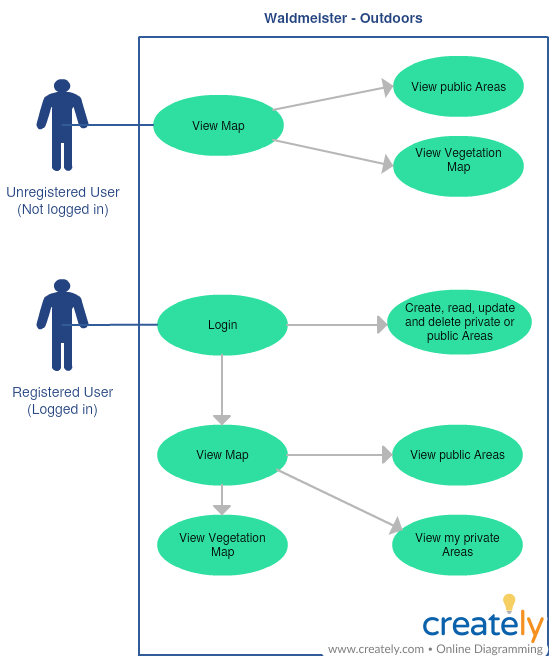
\includegraphics[width=0.7\textwidth]{WaldmeisterMap_USECASE}
    \caption{Use Cases}
    \label{fig:uc1}
\end{figure}


\section{Ergebnisse}
Nach einer Evaluation eines Prototyps, erstellt mithilfe eines kommerziellen Produkts,
und der Erstellung von Mockups, wurde ein eigenes Webapp 'Waldmeister Outdoors' realisiert. Durch diese App kann die Arbeit der Experten erleichtert werden. Da die Waldstandort-Karte gleichzeitig im Web synchronisiert
ist, wird dar\"uber hinaus der Informationsaustausch unter allen Beteiligten erleichtert. Die Webapp wurde f\"ur mobile Ger\"ate optimiert und die gew\"unschten Funktionen wurden umgesetzt. Registrierte Benutzer k\"onnen Benutzerfl\"achen in Form von Polygonen direkt auf der angezeigten Map erstellen, mit zus\"atzlichen Informationen versehen und auf einem Server speichern.

\begin{figure}[H]
\centering
    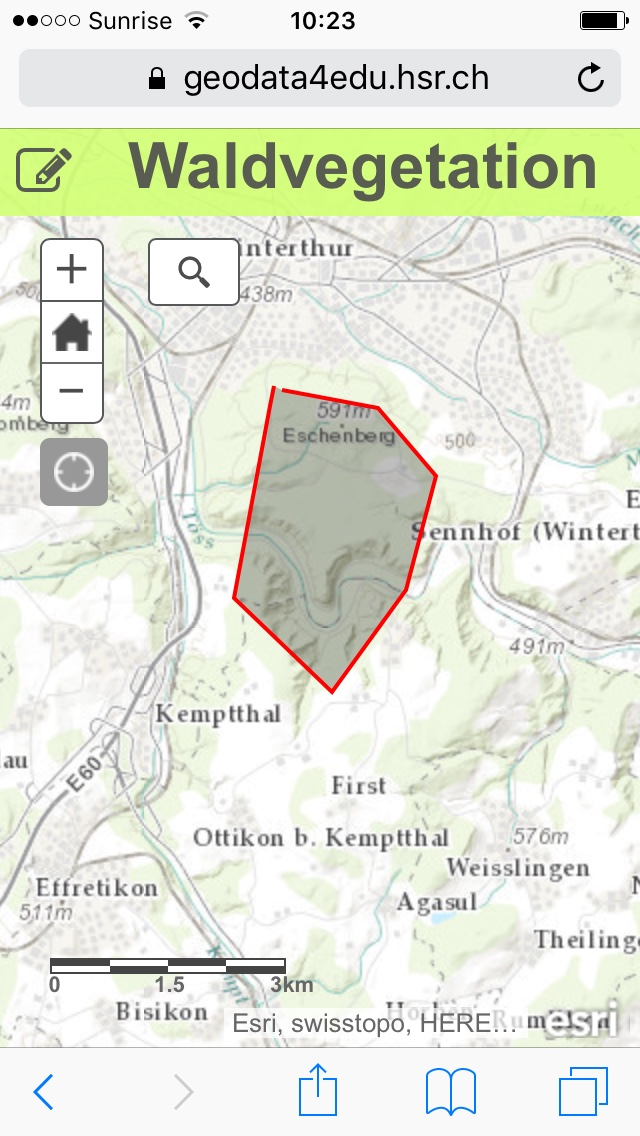
\includegraphics[width=0.3\textwidth]{esri-Waldvegetation2}
    \caption{ESRI Webapp Collector for ArcGIS}
    \label{fig:es1}
\end{figure}

\section{Ausblick}
Grosse Teile der Schweiz sind noch unkartiert, und viele Waldstandorte k\"onnten sich unter dem Einfluss der Klimaerw\"armung ver\"andern. Die kontinuierliche Beobachtung solcher Standorte ist Forschungsgegenstand von Forstingenieuren. Die Arbeit im Feld ist unerl\"asslich. "Waldmeister - Outdoors" kann im Berufsalltag sowie bei der Kommunikation mit Institutionen den Arbeitsfluss beschleunigen. Weitere Features k\"onnen dazukommen, wie die Verwendung von Plus Codes und offline-F\"ahigkeiten welche bei Verbindungsproblemen zum Einsatz kommen, bzw. Benutzerfl\"achen automatisch synchronisieren, sobald eine Verbindung besteht. Des weiteren bietet es sich an, dass sich User in Gruppen einklinken k\"onnen, um unter sich Benutzerfl\"achen zu teilen und zu besprechen, bevor sie ver\"offentlicht werden. Ebenfalls sollten erstellte Fl\"achen von registrierten Benutzern und deren Gruppen ver\"andert und gel\"oscht werden k\"onnen, nachdem sie erstellt wurden. $\newline$
"Waldmeister - Outdoors" hat das Potential in der Schweiz ein verbreitetes Tool zur Kartierung und Beobachtung von Waldfl\"achen zu werden und stellt eine bereits gefragte Erweiterung der beliebten "Waldmeister" App f\"ur mobile Ger\"ate dar.

\begin{figure}[H]
\centering
    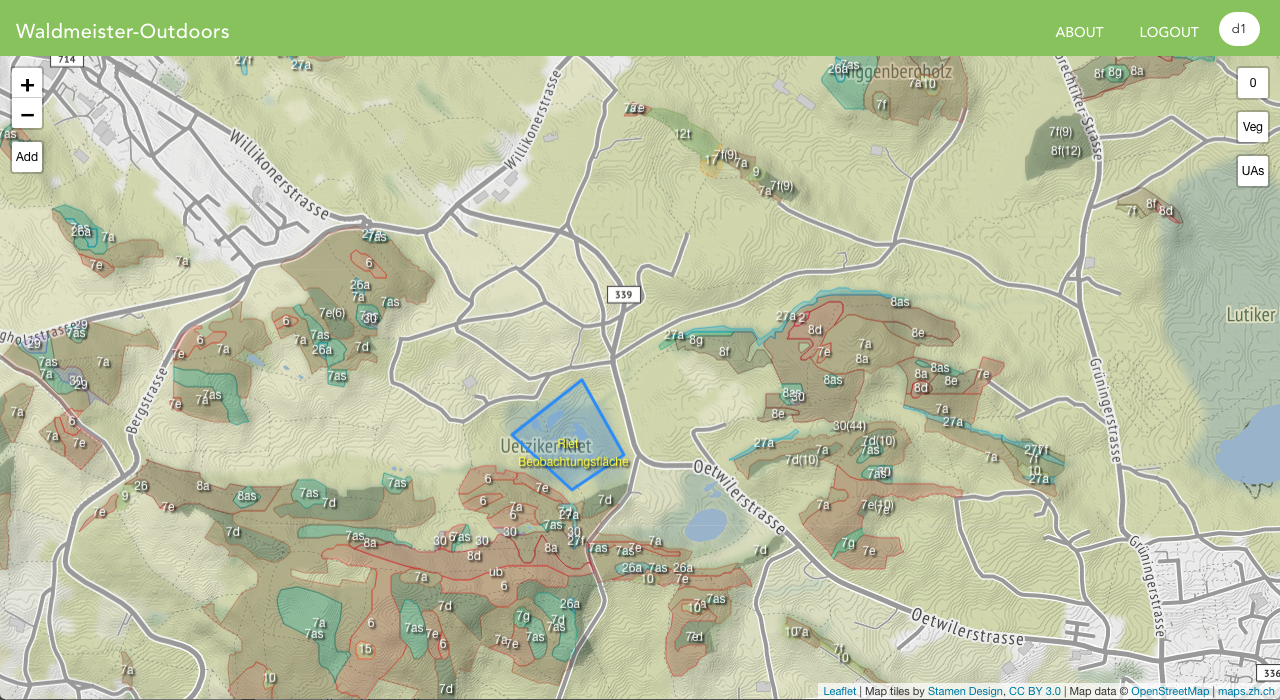
\includegraphics[width=1\textwidth]{RietBeobachtung3}
    \caption{Erfassung einer neuen Benutzerfl\"ache}
    \label{fig:es2}
\end{figure}

\renewcommand\thesection{\thechapter.\arabic{section}}

\chapter{Teil 1 - Technischer Bericht}
\section{Einf\"uhrung}

\subsection{Problemstellung, Vision}
Arbeit im Feld, wie sie bei der Kartierung von Waldstandorten unerl\"asslich ist, wird in allen F\"allen komplementiert von Arbeit, welche ausschliesslich im B\"uro erledigt werden kann. F\"ur viele Programme existieren ausschliesslich Desktop-L\"osungen, welche auf mobilen Ger\"aten nicht verwendet werden k\"onnen. Wie im Management Summary beschrieben, m\"ussen oft Arbeitsschritte im B\"uro wiederholt oder von Hand Niedergeschriebenes am Computer digitalisiert werden. K\"onnten diese Informationen bereits w\"ahrend der Feldarbeit digital festgehalten werde, w\"urde dies die Arbeit sehr verk\"urzen und den Informationsaustausch zwischen verschiedenen Personen und Teams einfacher gestalten. $\newline$
K\"onnen sich Personen und Teams untereinander bereits w\"ahrend der Arbeit im Feld \"uber Standorte austauschen, welche es zu kartieren gilt, k\"onnen sie sich freier und schneller im Feld organisieren und orientieren und so grossfl\"achige Projekte schneller bearbeiten. $\newline$
Kommt es zu einem sp\"ateren Zeitpunkt zu einer Revision von bereits kartierten Fl\"achen, kann bestehendes Kartenmaterial den Experten zur Verf\"ugung gestellt werden, welches sie auf mobilen Ger\"aten gleich im Feld analysieren und gegebenenfalls bearbeiten k\"onnen. Dies steht in einem starken Kontrast zum bestehenden Arbeitsfluss, welcher auf analogen Medien beruht.

\subsection{Ziele und Unterziele}
Ziel ist es, eine Webapp zu gestalten, welche es dem User erlaubt, bestehende Waldstandorte zu erforschen und nach Belieben neue Fl\"achen, welche Waldstandorte beschreiben k\"onnen, zu erfassen und zu editieren. Dies soll auf einem mobilen Ger\"at m\"oglich sein, welches im Feld verwendet wird. Die so erhobenen Daten sollen auf einem zentralen Server gespeichert und sofort dem User selbst sowie anderen Benutzern wieder zur Verf\"ugung gestellt werden. Daten, welche so im Feld eingegeben wurden, k\"onnen auch im B\"uro weiterbearbeitet werden. Um dies zu realisieren, wird eine Webapp mit einer Map erstellt, welche abh\"angig vom User dynamische Informationen auf der Map darstellt. 
Das technische Grundger\"ust der App besteht aus einem Client-Server, welcher dem User das Frontend liefert, und einem Backend, welches Daten vom User empf\"angt und speichert. Daten, welche von Usern erstellt werden, sollen an das Backend \"ubermittelt und in einer Datenbank persistent gemacht werden, damit sie von einem anderen Ger\"at aus oder von einem anderen User jederzeit zur Verf\"ugung stehen. Ausserdem erm\"oglicht es diese Architektur dem User einen Account zu erstellen und sich zu authentifizieren. $\newline$
Ziel ist es, dass die Map auf allen Ger\"aten dargestellt wird und dass nach erfolgreichem Login Fl\"achen in Form von Polygonen direkt auf der Map erstellt werden k\"onnen. Sie werden vom Backend persistent gemacht und mit dem eingeloggten Benutzer verkn\"upft. Der User kann danach auch auf anderen Ger\"aten auf diese erstellten Fl\"achen zugreifen und sie mit anderen Benutzern teilen.$\newline$

\subsection{Rahmenbedingungen}
Die Software soll auf mobilen Ger\"aten sowie auf Desktop/Laptop Browsern benutzbar sein. Mobile Ger\"ate sind von der Leistung her meist schwach verglichen mit Desktopger\"aten. Server-side rendering kann dieses Problem weniger relevant machen, weil damit die Applikation nicht vollst\"andig vom Client berechnet werden muss. $\newline$
Die Website ist darauf ausgelegt, dass sie im Chrome Browser verwendet wird, da Chrome der verbreitetste Browser auf Android Ger\"aten ist, und auch seine Desktop Version sehr zuverl\"assig funktioniert. Apple Ger\"ate k\"onnen ebenfalls Chrome verwenden. Chrome befindet sich auf den meisten Ger\"aten auf dem neusten Stand und unterst\"utzt daher die meisten Funktionen. $\newline$
Als Testger\"ate werden ein Apple iPad und iPhone verwendet, ein Android Galaxy S5 und mehrere Macbook Pro und Air Laptops (ca. Baujahr 2010 - 2016). $\newline$

\subsection{Vorgehen, Aufbau der Arbeit}
Es wurde eine Full-Stack Webapp aufbauend aus Frontend, Backend und Datenbank erstellt. Nach der Festlegung des Frontends wurde ein geeignetes Backend eruiert und die Datenbankanbindung f\"ur das Backend festgelegt. $\newline$
Als Frontend Framework wurde VueJS zur Erstellung von Single-Page-Applikationen gew\"ahlt. Als Backend kommt Django zum Einsatz, welches sich eignet um API Abfragen f\"ur das Frontend bereitzustellen. PostgreSQL wurde als Datenbank gew\"ahlt. $\newline$
Als erstes wurde das Loginsystem erstellt und im Frontend die verschiedenen Single-File-Komponenten entwickelt, damit User einen Account Registrieren und sich gegen\"uber dem Backend authentifizieren k\"onnen. $\newline$
Nachdem die Map Komponente erstellt wurde, konnten per API Abfragen die Benutzerfl\"achen geladen werden, welche im eingeloggtem bzw. nicht-eingeloggtem Zustand angezeigt werden. $\newline$
Danach wurden die Features implementiert und das Docker-Deployment vervollst\"andigt.

\pagebreak
\section{Stand der Technik}
\subsection{GIS-Browser}
Ein GIS-Browser, wie er von den verschiedenen Kanton in der Schweiz eingesetzt wird, ist ein read-only Archiv, bestehend aus \"offentlich zug\"anglichen Daten. Es k\"onnen verschidene Overlays ausgew\"ahlt werden, welche auf der Karte dargestellt werden, darunter auch die Vegetationskundliche Karte, auf welche in der Waldmeister-Outdoors Applikation zur\"uckgegriffen wird. 

\subsection{Collector for ArcGIS}
Technologien von ESRI (Environmental Systems Research Institute) und insbesondere ArcGIS online (GIS; Geografisches Informationssystem) wurden recherchiert, um einen funktionierenden Prototypen mit offline-caching zu erstellen. Hintergrundkarten (in Form eines Tile-Layers) k\"onnen auf dem Ger\"at zwischengespeichert werden. Die Erstellung von editierbaren Vektorlayern funktioniert auch im offline Betrieb und k\"onnen sp\"ater, sobald wieder eine stabile Internetverbindung besteht, synchronisiert werden. Dieses Verhalten kann bei einer Webapp durch Service-Worker rekreiert werden.$\newline$
Ein GeoJSON (Geo JavaScript Object Notation) file kann ebenfalls auf der online Plattform von ArcGIS hochgeladen werden und danach auf der Map dargestellt werden. Das Layer Styling kann so konfiguriert werden, dass die Farbe eines Polygons dem Typ des jeweiligen Waldstandorts entspricht.
$\newline$
Die Map und deren Inhalt wird im online Tool \href{https://geodata4edu.hsr.ch/}{geodata4edu} erstellt. Danach kann sie in der App Collector for ArcGIS (native App) verwendet werden. Feature Layer (oder gehostete Feature Layer) wie Areas und Points of Interest sind editierbar und synchronisieren mit dem Server sobald eine Internetverbindung besteht.

\begin{figure}[H]
    \centering
    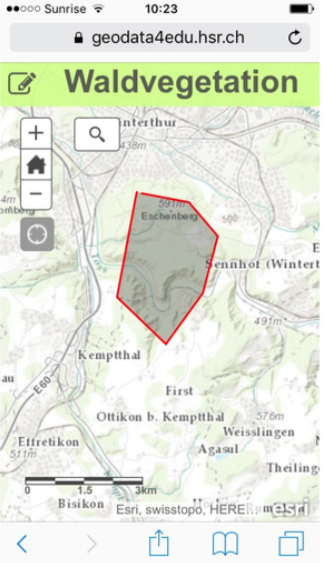
\includegraphics[width=0.5\textwidth]{esriprototyp}
    \caption{Prototyp mit ArcGIS online}
    \label{fig:mesh1}
\end{figure}

\subsection{Defizite}
Ein GIS-Browser, wie z.B. vom Kanton Z\"urich zur Verf\"ugung gestellt, bietet keine M\"oglichkeit, die eigene Position in Betracht zu ziehen, um damit den Kartenausschnitt zu bestimmen oder genauer noch, den aktuellen Waldstandortstyp per GPS zu bestimmen. Auch ist es nicht m\"oglich, pers\"onliche Notizen oder Fl\"achen wie Beobachtungsfl\"achen definieren, damit sie w\"ahrend der Arbeit im Feld verwendet werden k\"onnen. Dies liegt daran, dass sich ein User nicht identifizieren kann, und daher alle Benutzer bei jedem Besuch als anonym behandelt werden. Nur durch ein Loginsystem kann sich ein User gegen\"uber der Webseite gegen\"uber identifizieren und hat Zugriff auf von Ihm erstellten Informationen.$\newline$
Obwohl Collector for ArcGIS als ein sehr vielf\"altiges Werkzeug verwendet werden kann, hat es viele Nachteile, vorallem in Kombination ArcGIS online. Die Erstellung einer Map (Hintergrundkarte und Konfiguration der Feature Layer) ist sehr umst\"andlich und f\"ur User, welche sich nicht mit den Tools auskennen, nicht ersichtlich. Zum Beispiel mussten gewisse Layer, damit sie korrekt funktionierten, mithilfe der Webseite developers.arcgis.com/ erstellt werden, um sie danach in der Map, welche auf ArcGIS online zusammengeklickt wird, zu importieren. Auf developers.arcgis muss zum Erstellen dieser Layer ein Enterprise Account benutzt werden, welcher eine Organization URL ben\"otigt. Da diese Layer in der ArcGIS online Map und danach in der mobile App "Collector for ArcGIS" verwender werden, ben\"otigen auch Enduser diesen Login, was eine Verbreitung der App verunm\"oglicht. Benutzer, welche keinen Enterprise Login haben, k\"onnen bei ArcGIS online lediglich "Public Accounts" erstellen. Diese sind aber in der Funktionalit\"at eingeschr\"ankt.

\section{Bewertung}
\subsection{Kriterien}
Funktionalit\"at $\newline$
Maps.zh.ch eignet sich sehr gut um Zugriff auf das sehr umfangreiche Kartenmaterial-Archiv des Kantons zu erhalten. Die Karten sind jedoch als read-only Archiv eingerichtet und auf der Map, welche von maps.zh.ch bereitgestellt wird, lassen sich keine digitalen Anmerkungen, Kommentare oder eigene Fl\"achen oder Points of Interests anbringen. Informationen \"uber eine spezifische Eigenschaft der aktuellen Position im Feld zu erhalten, kann jedoch sehr zeitintensiv sein, da die richtige Karte eingeblendet werden muss und auf der Map manuell an den richtigen Ort hingepant und hineingezoomt werden muss. Da die eigene Position auf der Map nicht ersichtlich ist, muss oft die eigene Position in einem anderen Tool berechnet werden (zum Beispiel Google Maps), um danach per Informationen \"uber einen gew\"ahlten Ort zu erhalten. Maps.zh.ch stellt keine API bereit, welche es erm\"oglicht, Abfragen zu einen gegebenen Ort auszuf\"uhren oder Kartenmaterial wie zum Beispiel die Waldvegetationskarte auf einer anderen Map darzustellen. Kartenmaterial muss gekauft und darf nur unter Einhaltung der Nutzungsbedingungen verwendet werden. $\newline$
$\newline$
Eine native App wie "Collector for ArcGIS" eignet sich, um eine Datensammler Applikation zu erstellen. Das Loginsystem sollte jedoch vereinfacht werden und keine Accounts ben\"otigen, welche an andere Unternehmen gebunden sind. Die Webapp Waldmeister-Outdoors soll ein eigenst\"andiges Projekt werden, welches keine Vorkonfigurierten Map Eigeschaften beinhaltet, welche von in einem Web-Editor wie ArcGIS online erstellt worden sind.

\subsection{Schlussfolgerungen}
Waldmeister-Outdoors kann ein Karten-Archiv wie maps.zh.ch anbietet stark aufwerten und durch ein Login System erweitert werden. User sollen wie im "Collector for ArcGIS" die M\"oglichkeit haben neue Objekte wie Fl\"achen und Points of Interest zu erstellen und Positionsabh\"angige Funktionen wie den Kartenausschnitt zu zentrieren und den eigenen Standort anzuzeigen. Dies soll \"uber GPS Funktionen von internetf\"ahigen (Mobilen) Ger\"aten erm\"oglicht werden und in der Map reflektiert werden.

\section{Umsetzungskonzept}
\subsection{L\"osungsans\"atze}
Damit die App auf mehreren Ger\"aten mit unterschiedlichen Betriebsystemen verwendet werden kann, bietet es sich an eine Webapp zu verwenden, welche in Internet auf einer URL aufgerufen wird. Im Gegensatz zu einer nativen ist diese Webapp plattformunabh\"angig und muss nicht auf native Umgebungen angepasst werden, da sie vom jeweiligen Browser des Ger\"ats interpretiert wird. $\newline$
 Um die geplanten Funktionalit\"aten wie das Login und das Erstellen von Benutzerfl\"achen umzusetzen, muss die Webapp einer 3-Tier Architektur entsprechen, welche auf Frontend, Backend und einer Datenbank aufbaut. 
$\newline$
\subsection{Frontend}
Der Frontend-Client soll als Webapp realisiert werden. Daf\"ur soll ein modernes Webframwork gew\"ahlt werden, welches zur Erstellung einer Single-Page-Applikation (SPA) eingesetzt wird. Waldmeister-Outdoors soll f\"ur Browser von Mobilen und Desktop Ger\"aten optimiert werden, wie zum Beispiel Chrome oder Firefox. 
\subsection{Backend}
Als Backend soll ein flexibles Framework, welches Micro-Services und API Abfragen in Form von REST-Schnittstellen bereitstellen kann, eingesetzt werden. Django wurde gew\"ahlt, da es von vielen Projekten des IFS bereits erfolgreich eingesetzt wurde.
\subsection{Datenbank}
PostgreSQL ist ein open-source Datenbank Management System. Es ist dank der PostGIS Erweiterung sehr gut geeignet um raumbezogene Daten (Geospacial Data), wie die Daten der Vegetationskundlichen Karte, zu storen und ab zu fragen.
\subsection{JavaScript Libraries und Node Module}
Leaflet editable $\newline$
Damit die User neue Polygone, Punkte und Pfade erfassen k\"onnen, wird die Library "Leaflet editable" verwendet. Es erm\"oglicht, neue Objekte (zum Beispiel Polygone und PoIs) direkt auf der Leaflet Map zu zeichnen, oder bestehende Objekte zu editieren. $\newline$
Vuetify $\newline$
Vuetify ist ein Node Module welches als offzielle Material-Design-Extension von VueJS behandelt wird. Es stellt es viele UI - Komponenten bereit, welche in einer VueJS Applikation verwendet werden k\"onnen.  $\newline$
$\newline$
Eine vollst\"andige Liste der Node Module befindet sich in der Datei package.json im Ordner client.
\subsection{Python Pakete}
Die wichtigsten Python Pakete sind Django 2.0, welches das Grundger\"ust des Backend-Servers darstellt. Django verwendet als Server das Python Paket Djangorestframework 3.8.2 um API Requests des Frontends zu beantworten. $\newline$
Eine komplette Liste der Verwendeten Python Pakete wird in der file Requirements.txt des backends gef\"uhrt.
\subsection{Werkzeuge und Tools}
Als IDE bzw. Texteditor wurde das Programm Sublime 2 verwendet, welches die beiden Linter Eslint (f\"ur JavaScript Code) und flake8 (f\"ur Python Code) unterst\"utzt. Entwickelt wurde auf einer lokalen Node und Python Umgebung, bzw. in dockerisierter Form, um das deployment zu testen.
\subsection{Deployment}
Das Projekt soll auf einem HSR Server deployt werden, damit es per URL im Internet erreichbar ist.

\section{Resultate}
\subsection{Zielerreichung}
User k\"onnen mittels der Webapp Waldmeister-Outdoors die Vegetationskundliche Karte erforschen und diese mit Ihrem momentanen Standort abgleichen. Dar\"uber hinaus k\"onnen sie, nachdem sie sich registriert haben, private und \"offentliche Benutzerfl\"achen auf einem mobilen Ger\"at erfassen und sie auf einem zentralen Server hinterlegen. Somit k\"onnen sie pers\"onliche Orte und Fl\"achen erstellen, welche f\"ur Sie im Arbeitsalltag relevant sind und sie zwischen verschiedenen Ger\"aten (Im Feld und im B\"uro) abrufen oder mit anderen Personen teilen. Erstellte Benutzerfl\"achen k\"onnen zu einem sp\"ateren Zeitpunkt oder von einem anderen Ger\"at aus editiert oder gel\"oscht werden.$\newline$
Ebenfalls erreicht wurde die Geolocation auf der Karte zu repr\"asentieren. Dies ist im Arbeitsalltag eine grosse Hilfe, und dient zur schnellen Orientierung und Auffindung von bestimmten eingetragenen Fl\"achen und Orten im Feld. Die GPS-Position wird mit einem gesetzten Intervall von f\"unf Sekunden erneuert, und die erhaltenen Koordinaten werden auf der Map als Element, bestehend aus zwei Circles, dargestellt. $\newline$
Die Webapp kann sowohl auf Desktop Browsern wie von mobilen Ger\"aten verwendet werden und verh\"alt sich dank VueJS responsive auf eine \"Anderung des Viewports, zum Beispiel wenn der Screen eines mobilen Ger\"ats w\"ahrend der Verwendung gedreht wird. $\newline$
Layer und deren Label k\"onnen ein - und ausgeblendet werden, was zur \"Ubersicht beitragen kann. $\newline$
Alle Benutzeraccounts und deren Fl\"achen sind im Django Backend ersichtlich und k\"onnen als Superuser ver\"andert oder gel\"oscht werden. Wird ein Benutzer aus der Datenbank gel\"oscht, werden alle von ihm erstellten Benutzerfl\"achen ebenfalls automatisch gel\"oscht. Alle Passw\"orter von Benutzeraccounts werden gehasht in der Datenbank gespeichert. $\newline$
Die Webapp wurde auf dem IFS Server als Dockerimage deployt und ist im Internet erreichbar unter \href{https://waldmeistermap.sifs0003.infs.ch/}{Waldmeister-Outdoors} .

\subsection{Ausblick}
Als Wichtigste Punkte zur Weiterentwicklung der Webapp ist die Implementierung einer Vegetationslayer-API, welche das dynamische Laden von Waldstandortsfl\"achen des Clients erm\"oglicht. $\newline$
Anpassungen an des UI und weitere Funktionen im Frontend welche die Zusammenarbeit im Team verbessert sollten ebenfalls realisiert werden. $\newline$
Genauere Ausf\"uhrungen zur Weiterentwicklung befinden sich im Kapitel 4.9.2 der Projektdokumentation.

\subsection{Pers\"onliche Berichte}
W\"ahrend der Entwicklung wurde ein Update f\"ur das Ubuntu Basisimage ver\"offentlicht, welche die ben\"otigten Libraries von Gdal \"anderte. Gdal (GDAL - Geospatial Data Abstraction Library) setzt diese daf\"ur ein, Geodaten zwischen verschiedenen Formaten zu konvertieren. Die verwendete Version (welche im Dockerfile definiert wird) muss jedoch der Version der Hostmachine von Docker entsprechen. Dieses Update kam zu einem \"uberraschenden Zeitpunkt, und der Build konnte w\"ahrend dieser Zeit nicht ausgef\"uhrt werden, bis dass Problem gefunden und behoben wurde. Das Problem wurde erst bemerkt, als das Build von Travis ausgef\"uhrt wurde, da die lokale Entwicklung des Build davon nicht beeintr\"achtig waren (da in der lokalen Entwicklung kein Ubuntu eingesetzt wurde). Travis ist hier eine grosse Hilfe ein Build auf einem anderen Computer zu testen, bevor die Version live auf dem produktiven Server deployt wird, was in diesem Fall zu einem Unterbruch des Services gef\"uhrt h\"atte.

\clearpage
\pagebreak


\chapter{Teil 2 - SW-Projektdokumentation}
\section{Anforderungsspezifikation}
\subsection{Use-Cases}
W\"ahrend der Feldforschung kann es sehr hilfreich sein, auf bereits kartierte Waldfl\"achen Zugriff zu haben, um sich am Standort zu orientieren. Dieses Material ist oft in einem Kantonalen Portal z.B. \href{https://maps.zh.ch}{maps.zh.ch} erh\"altlich, es ist jedoch nur selten kompatibel mit mobilen Ger\"aten, interagieren nicht mit dem GPS des Smartphones oder die Websiten sind schwer zu navigieren. "Waldmeister - Outdoors" soll einem gezielten Zweck dienen und nicht mit Kartenmaterial \"uberladen werden. Der Zugriff auf die Vegetationskundlichen Karten sollte vereinfacht und die Navigation beschleunigt werden. $\newline$
Der \"uber GPS ermittelte eigene Standort soll auf der Karte eingetragen werden und beim Laden der Map soll auf diesen Kartenausschnitt  zentriert werden. Diese Funktion des Zentrieren kann jedoch beim Erforschen von Waldstandorten, welche sich nicht in unmittelbarer N\"ahe befinden als st\"orend empfunden werden. Daher sollte diese Funktion deaktivierbar sein, oder nur einmalig beim Laden der Map ausgef\"uhrt werden. $\newline$
Durch einen Abruf in der Datenbank kann ermittelt werden, ob sich der Benutzer zu diesem Zeitpunkt gerade innerhalb eines Waldstandorts befindet, falls sich die ermittelte Position des Ger\"ats innerhalb eines Polygons befindet, welches in der Vegetationskarte gespeichert ist. Dies soll dem User auf der Map jederzeit mittgeteilt werden, auch wenn er sich zum Zeitpunkt nicht auf dem Kartenausschnitt sichtbar ist.

\subsection{Use Case - Diagramm}
Das Diagram \ref{fig:uc1} zeigt auf, welche M\"oglichkeiten ein User hat, mit dem Werkzeug zu interagieren. Ein User, welcher sich nicht registriert, kann keine Fl\"achen generieren oder editieren und kann auch keine privaten Fl\"achen sehen. Er kann jedoch die Vegetationskundliche Karte und \"offentliche Fl\"achen aller anderen User sehen. $\newline$
Nachdem er sich registriert und eingeloggt hat, kann er Fl\"achen erstellen und editieren. Diese teilen sich in \"offentliche und private Benutzerfl\"achen auf. Diese Option kann er w\"ahrend der Erfassung der Geometrie der Fl\"ache frei w\"ahlen. Standardm\"assig ist eine solche Fl\"ache privat und wird nur auf Wunsch des Users \"offentlich gemacht. Eine bereits erstellte Fl\"ache kann aber im Nachhinein auf \"offentlich umgeschaltet werden, nachdem sie z.B. durch \"Anderungen der Geometrie und Position vom User finalisiert wurde. Dies ist vorallem nach Absprache zwischen anderen Experten denkbar, welche \"uber Gruppen auch auf private, noch nicht \"offentliche Benutzerfl\"achen Zugriff haben um die Eigenschaften und Lage einer Fl\"ache zu analysieren und \"uber diese zu diskutieren.
\begin{figure}[H]
\centering
    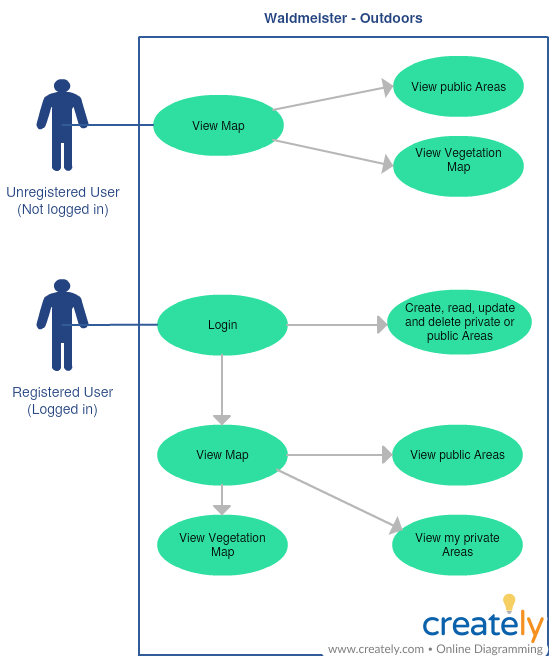
\includegraphics[width=0.9\textwidth]{WaldmeisterMap_USECASE}
    \caption{Use Case Diagram}
    \label{fig:uc1}
\end{figure}

\subsection{Must-Haves}
Als must-haves werden funktionale Anforderungen beschrieben, welche zentrale Funktionen beschreiben, welche ein User mit der Applikation durchf\"uhren m\"ochte. Dazu geh\"oren die Navigation der Map und das Erstellen und Editieren von Benutzerfl\"achen. Ein Login, bzw Registrierungsvorgang ist dabei unerl\"asslich, damit sich User authentifizieren k\"onnen, auf welches Kartenmaterial sie Zugriff haben. Bei Benutzerfl\"achen wird hierbei unter pers\"onlichen (privaten) und \"offentlichen Benutzerfl\"achen unterschieden. $\newline$
API-Abfragen sollen wo m\"oglich gesch\"utzt werden und Benutzerfl\"achen, welche von einem User erstellt wurden, sollen nicht von anderen Usern ver\"andert oder gel\"oscht werden k\"onnen. $\newline$
Das Projekt soll per Docker-Container auf dem IFS Server deployt werden und per Link f\"ur Jedermann zug\"anglich sein.

\subsection{Optional}
Als optionale Anforderung wurde die Automatische Anzeige des Waldstandorttyps bezeichnet. Neben der Map, welche alle Waldstandorte am geografisch korrekten Ort darstellt, ist eine ortsbasierte Anzeige des momentanen Waldstandortstypen hilfreich bei der Arbeit im Feld. Diese Anzeige besteht daraus, die GPS Position des Ger\"ats zu verwenden, um in einer Datenbank zu ermitteln, ob der ermittelte Punkt innerhalb eines bekannten Waldstandorts liegt.

\subsection{Nicht-funktionale Anforderungen}
Die Software soll auf mobilen Ger\"aten sowie auf Desktop/Laptop Browsern benutzbar sein. Mobile Ger\"ate sind von der Leistung her meist schwach verglichen mit Desktopger\"aten. Server-side rendering kann dieses Problem weniger relevant machen, damit die Applikation nicht vollst\"andig vom Client berechnet werden muss. $\newline$
Die Website ist darauf ausgelegt, dass sie im Chrome Browser verwendet wird, da Chrome der verbreitetste Browser auf Android Ger\"aten ist, und auch seine Desktop Version sehr zuverl\"assig funktioniert. Apple Ger\"ate k\"onnen ebenfalls Chrome verwenden. Chrome befindet sich auf den Meisten Ger\"aten auf dem neusten Stand und unterst\"utzt daher die meisten Funktionen. $\newline$
Als Testger\"ate werden ein Apple iPad und iPhone verwendet, ein Android Galaxy S5 und mehrere Macbook Pro und Air Laptops (ca. Baujahr 2010 - 2016). $\newline$
Ziel ist es, dass die Map auf allen Ger\"aten dargestellt wird und nach erfolgreichem Login Fl\"achen in Form von Polygonen direkt auf der Map erstellt werden k\"onnen. Sie werden vom Backend persistent gemacht und mit dem eingeloggten Benutzer verkn\"upft. Der User kann danach auch auf anderen Ger\"aten auf diese erstellten Fl\"achen zugreifen und sie mit anderen Benutzern teilen.$\newline$

\pagebreak
\section{Domain Modell}
Das Diagramm \ref{fig:cd1}  schildert die Relation und den Ausbau der wichtigsten Klassen des Systems. Dies zeigt, dass Benutzerfl\"achen nur von registrierten Usern erstellt werden k\"onnen und immer einem solchen zugewiesen sind. Wird ein Benutzer aus dem System gel\"oscht, werden alle Fl\"achen welche diesem Account zugeordnet sind , ebenfalls aus dem System gel\"oscht. $\newline$
Die Waldvegetationsfl\"achen sind in der Datenbank als Modell bestehend aus Polygon und einem String mit dem Waldstandortstypen nach EK72 gespeichert. Beim Starten des Backends werden sie aus einem Shapefile geladen und in der Datenbank persistent gemacht, sofern sich der Datensatz nicht bereits in der Datenbank befindet.

\begin{figure}[H]
\centering
    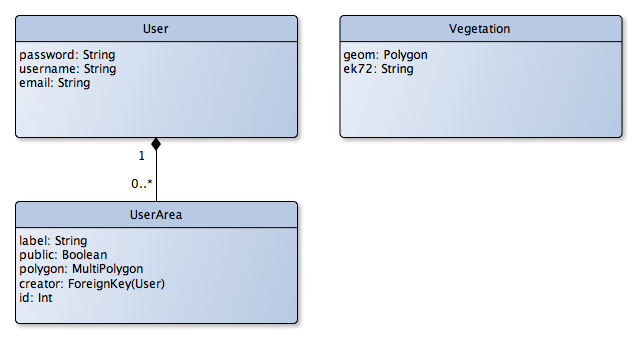
\includegraphics[width=1\textwidth]{DomainModell2018}
    \caption{Domain Modell}
    \label{fig:cd1}
\end{figure}


\section{Technologien}
\subsection{Django}
Als Server zur Verwaltung der User und der Daten, welche die User generieren und ben\"otigen, kommt Django zum Einsatz. Es ist ein Open-Source Webframework, welches das Python Gegenst\"uck zu Ruby-On-Rails darstellt. Im Kern folgt es dem Model-View-Controller Prinzip, obwohl es eine eigene Namensgebung verwendet. \cite{django1} In diesem Projekt verwendet Django eine PostgreSQL Datenbank um Daten persistent zu machen. Django wird ebenfalls dazu verwendet, um User einen Account zu geben, damit nur sie selbst Zugriff auf Ihre privaten Benutzerfl\"achen haben, oder um \"offentlich erstellte Benutzerfl\"achen mit anderen zu teilen. Zur Authentifizierung wird ein JWT eingesetzt. $\newline$

\subsubsection{Django Rest Framework}
Eine SPA kommuniziert haupts\"achlich \"uber API Schnittstellen mit dem Server. Hier kommt auf dem Server das Django Rest-Framework (DRF) zum Einsatz. $\newline$
Es bietet ein sehr flexibles System zur Erstellung von RESTful Web-APIs. Das DRF bietet die M\"oglichkeit CRUD Operationen auf eine Ressource auszuf\"uhren. "Waldmeister - Outdoors" verwendet die REST Api beispielsweise um usergenerierte Fl\"achen, Pfade oder Punkte in der Datenbank zu speichern oder diese zur Darstellung in der Map aus der Datenbank zu laden. $\newline$
Ebenfalls werden Benutzer, welche sich registrieren, mit Username, Password und ggf. Emailadresse in der Datenbank eingetragen. $\newline$

\subsection{PostgreSQL}
Postgres ist das Datenbank Management System, welches mit Django zusammen die Daten persistent macht, welche die User per API in der PWA generieren. Hierzu wird das Django Packet psycopg2 verwendet. Django kann durch Models ein Datenbankschema beschreiben, welches von PostgreSQL generiert und in einer lokalen PostgreSQL Instanz gespeichert wird. \cite{pg1} \cite{django2}

\subsubsection{PostGIS}
Um Geoinformationsdaten wie z.B. Polygone und Pfade korrekt zu speichern wird auf der Datenbank das Plugin PostGIS installiert. Dadurch kann Django die ben\"otigten Datenbankmodelle erstellen und per REST Schnittstelle speichern. Anhand des Django Models werden Geodaten in einem gew\"ahlten Format gespeichert. Standardm\"assig wird von Django die Spatial Reference Identifier (SRID) Nummer 4326 (World Geodetic System, WGS84) verwendet. Dieses System benutzt Zahlen von -180, -90 bis 180, 90 um Positionen auf der Erde (in Latitude und Longitude) zu beschreiben. $\newline$
Postgis wird ebenfalls dazu verwendet, dass die Daten, welche per REST-Schnittstelle an den Client geschickt werden, in richtigem Format (Multipolygone in GeoJSON) \"ubermittelt werden.

\subsection{VueJS}
Vue.JS ist ein JavaScript Framework, welches sich zum Erstellen von Single-Page-Webapplikationen in Form einer PWA eignet. Es wurde im Jahr 2013 erstmals ver\"offentlicht und wurde am 19. Dezember 2017 auf die aktuellste Version 2.5.13 gepatcht. Vue.JS folgt einer Variation des Model-View-Controller-Entwurfmusters, dem Model - View - ViewModel Muster. Wie auch das MVC dient MVVM der Trennung von Darstellung und der Logik der Benutzerschnittstelle. Dies erlaubt dem nutzenden Entwickler, die Struktur der Anwendung nach eigenen Anspr\"uchen zu richten. $\newline$
Entwickler beschreiben es daher als "less opinionated" im Vergleich zu anderen popul\"aren JavaScript Webframeworks wie Anglar.JS oder React. Vue.JS kann von Entwicklern eingesetzt werden, welche HTML und JavaScript beherrschen und erfordert keine weiteren Webtechnologien. Vue.JS setzt eine Website aus Instanzen und Komponenten, bzw Single File Components zusammen. Single File Components sind bei VueJS, welche Architekturprobleme von mittel bis grossen Webapps, welche vollst\"andig von JavaScript getrieben werden, zu verbessern versucht. $\newline$
Folgende Probleme tauchen dabei auf:
$\newline$
\begin{enumerate}
\item Global definitions $\newline$
Global definitions force unique names for every component
\item String templates $\newline$
String templates lack syntax highlighting and require ugly slashes for multiline HTML
\item No CSS support $\newline$
No CSS (Cascading Style Sheets) support means that while HTML and JavaScript are modularized into components, CSS is conspicuously left out
\item No build step $\newline$
No build step restricts us to HTML and ES5 JavaScript, rather than preprocessors like Pug (formerly Jade) and Babel
\end{enumerate}
$\newline$
VueJS besagt, dass all diese Probleme von Single File Components (mit .vue extension) dank Werkzeugen wie Webpack und Browserify gel\"ost werden. Eine solche Komponente besteht auf HTML Template, JavaScript und CSS in einer eigenen, abgekapselten Datei. 
$\newline$
Durch das erzielt VueJS $\newline$

\begin{enumerate}
\item Complete syntax highlighting
\item CommonJS modules
\item und Component-scoped CSS
\end{enumerate}

Wem diese Idee Abkapselung nicht gef\"allt, der kann weiterhin ein CSS auslagern und in eine Komponente (innerhalb des HTML Templates) importieren: $\newline$
\begin{lstlisting}
<!-- my-component.vue -->
<template>
  <div>This will be pre-compiled</div>
</template>
<script src="./my-component.js"></script>
<style src="./my-component.css"></style>
\end{lstlisting}
$\newline$

\subsubsection{Separation of Concern}
Was ist gemeint mit Separation of Concern (SoC) und bricht der Aufbau von Single-File-Components nicht dieses Pattern? Eine bekannte Vorgehensweise bei Softwareengineering ist es, ein Computerprogramm in logische Abschnitte einzuteilen und zu separieren. Diese Teile sollten sich um einen Zweck oder Belang (Concern) k\"ummern. Dies heisst jedoch nicht, dass die verschiedenen Dateitypen unbedingt in separate Dateien aufgeteilt werden. In der modernen User-Interface-Entwicklung und den Entwicklern von VueJS ist es oft leichter gefallen, verschiedene Komponenten, welche lose gekoppelt sind, zu komponieren, statt sie auf drei riesigen Layern (HTML, JS und CSS) getrennt zu halten, sie aber in den Komponenten zu verflechten. \cite{VueSFC} $\newline$
Auf diesem Weg sind Komponenten (Template, die Logik und das Styling) zusammenh\"angender und auch einfacher zu warten, obwohl dies nicht den Prinzipien von SoC folgt. Traditionelles SoC unterteilt dies in die Gruppen der Zwecke Organisation (HTML), Pr\"asentation (CSS) und Interaktion bzw. Verhalten (JavaScript).

\subsubsection{Vue-Router}
Der Vue-Router ist das Herzst\"uck einer Single-Page-Applikation (SPA). Der offizielle Vue-Router ist ein Client-seitiger Router, welcher mithilfe der HTML5 History API voll funktionsf\"ahiges Client-side routing macht. $\newline$ In der HTML Definition der Hauptkomponente kann <router-view> als Platzhalter verwendet werden, um die Komponenten anzuzeigen, welche abh\"angig von der momentanen Route an dieser Stelle angezeigt werden sollen. Ein Wechsel zwischen diesen Routen bewirkt kein Page-Reload, da dies von Vue.JS lediglich innerhalb derselben Page \"Anderungen bewirkt und keine tats\"achlichen URL Aufrufe ausf\"uhrt. $\newline$
Der Vue Router wird innerhalb einer Hauptseite angezeigt welche die Basis der Webseite darstellt. Methoden von Komponenten k\"onnen bewirken, dass sich der Inhalt ver\"andert, welcher an der Stelle des Router-Views angezeigt wird. Menupunkte im Header (z.B Register, Login, About, Map), bewirken mit .push() dass der Vue-Router mithilfe des index.js files die korrekten Komponenten an dieser Stelle anzeigt. Dies kann auch direkt \"uber eine URL Eingabe /register oder /login erfolgen, ohne dass der Aufruf \"uber eine interne Komponente ausgef\"uhrt werden muss. Die Datei index.js beinhaltet daher alle m\"oglichen Pfade, welche von der Webapp aufgel\"ost werden und bestimmt die angezeigten Komponenten, welche mit dieser Route verkn\"upft sind. $\newline$
Alternativ k\"onnten die \"ahnlichen L\"osungen von Page.js oder Director als Third-Party Produkte an dieser Stelle integriert  werden, es ist jedoch zu empfehlen, die offizielle Vue-Router Library zu verwenden.

\subsubsection{VueX}
VueX ist eine offizielle Erweiterung von Vue.JS und fungiert als Statusmanager. VueX arbeitet mit einem Store, welcher die Zust\"ande aller Komponenten in einer Vue Applikation \"uber Regeln definiert. VueX besteht aus Actions, Mutations und States. Aktionen k\"onnen in dieser Reihenfolge eine Auswirkung auf die Vue Komponenten haben. $\newline$
VueX hat Vorteile bei mittel bis grossen Projekten, welche auf dem Single-Page-Application Prinzip basieren. VueX bietet auch die M\"oglichkeit, einen zentralen Store in kleinere Module aufzuteilen, jedes mit ihren eigenen State, Mutations, Actions Werten. $\newline$
Da Komponenten in Vue abgekapselt sind, k\"onnen sie standardm\"assig nicht auf Daten zugreifen ,welche in anderen Komponenten definiert werden. Solche Daten m\"ussen per Store verf\"ugbar gemacht werden, damit sie \"uber mehrere Instanzen geteilt werden k\"onnen. $\newline$

\begin{lstlisting}
const sourceOfTruth = {}

const vmA = new Vue({
  data: sourceOfTruth
})

const vmB = new Vue({
  data: sourceOfTruth
})
\end{lstlisting}
$\newline$

Wird nun sourceOfTruth ver\"andert, wird sie in allen Komponenten, in welcher sie verwendet wird, automatisch auf den neuen Stand gebracht. Dies kann in gr\"osseren Applikationen schnell un\"ubersichtlich werden, da jede Komponente diese sourceOfTruth ver\"andern kann, ohne eine nachvollziehbare Spur zu hinterlassen. Es wird daher empfohlen, das Store Pattern von VueX zu implementieren, welche Ver\"anderungen am Store nur \"uber Mutationen zul\"asst. Somit wird es klarer, zu welcher Zeit welche Mutationen aufgerufen werden k\"onnen und wie sie durchgef\"uhrt wurden:$\newline$

\begin{lstlisting}
var store = {
  debug: true,
  state: {
    message: 'Hello!'
  },
  setMessageAction (newValue) {
    if (this.debug) console.log('setMessageAction triggered with', newValue)
    this.state.message = newValue
  },
  clearMessageAction () {
    if (this.debug) console.log('clearMessageAction triggered')
    this.state.message = ''
  }
}
\end{lstlisting}
$\newline$

\begin{figure}[H]
    \centering
    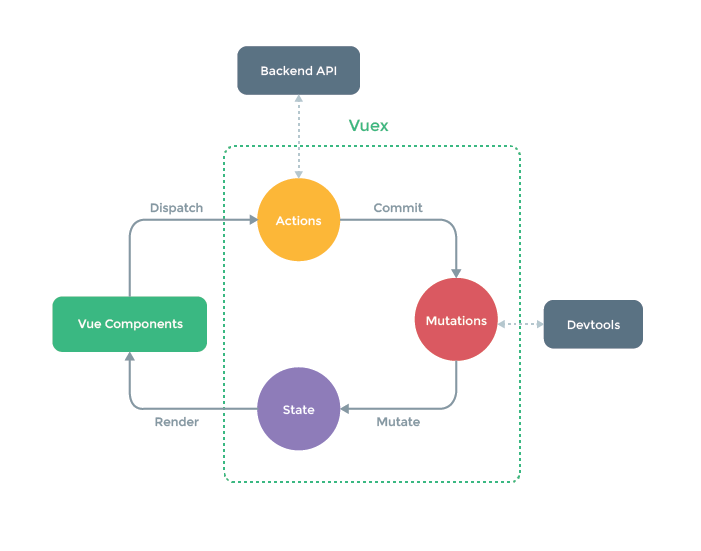
\includegraphics[width=1\textwidth]{vuex}
    \caption{Vuex Action-Mutations-State Diagram}
    \label{fig:mesh1}
\end{figure}
$\newline$
Komponenten k\"onnen auch private Zust\"ande haben, dies wird mit "privateState" erreicht. In diesem Fall muss der sharedState ebenfalls definiert werden.

\begin{figure}[H]
    \centering
    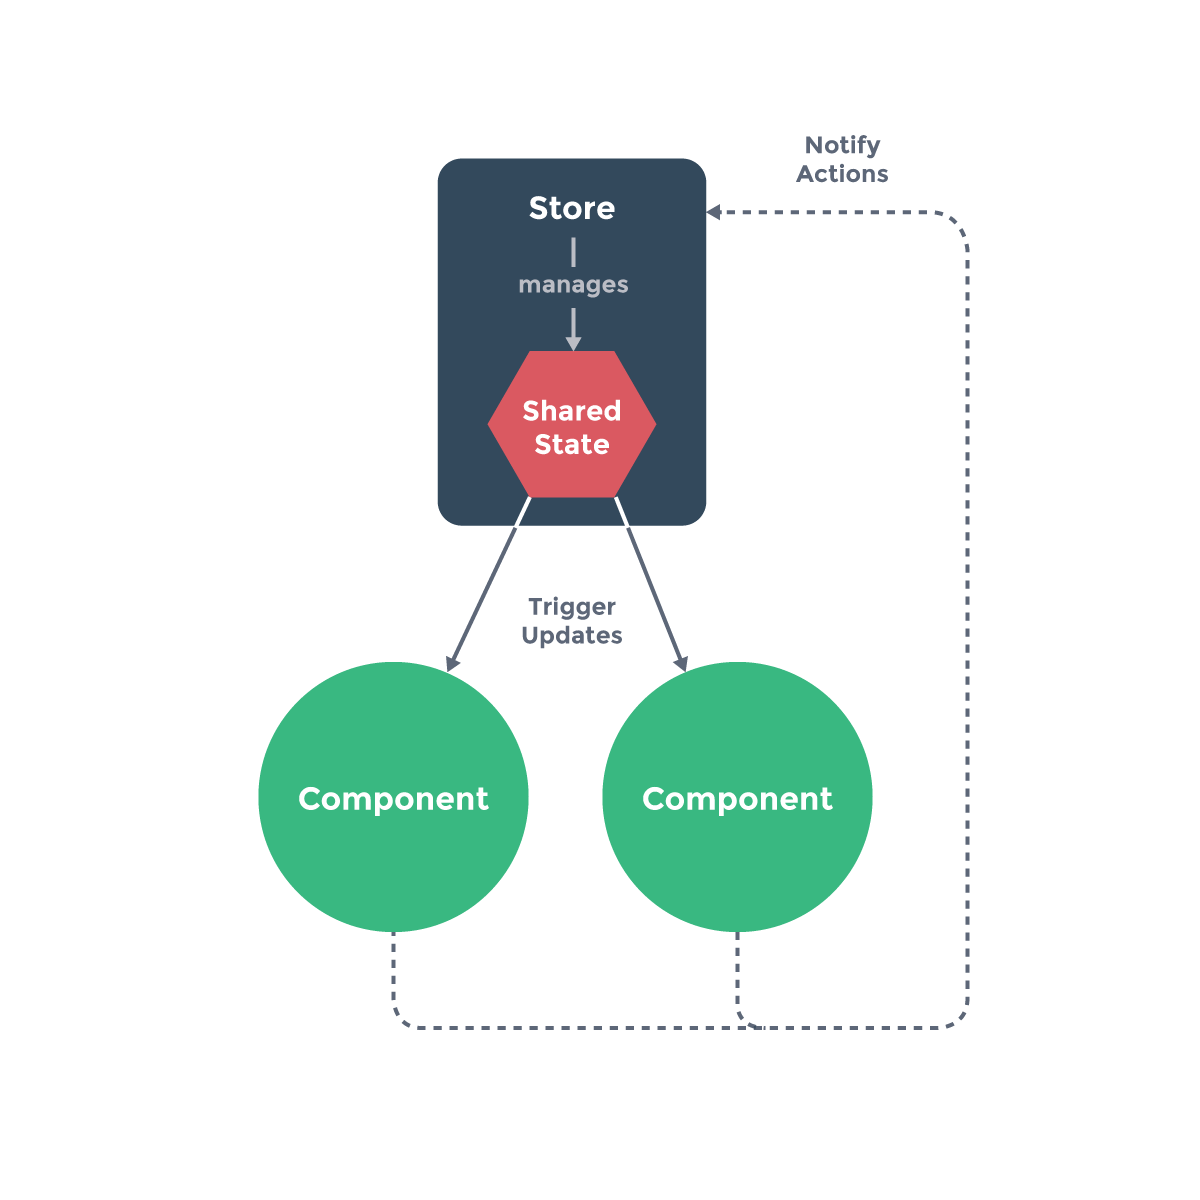
\includegraphics[width=0.7\textwidth]{sharedstate}
    \caption{Vuex private}
    \label{fig:mesh2}
\end{figure}
$\newline$
Dies bewirkt, dass eine Komponente nicht direkt einen Wert oder Zustand im Store ver\"andern kann, sondern dies einen Event aufruft. Dieser informiert den Store welchen State es \"uber eine Mutation zu ver\"andern gilt.

\subsection{Docker}
Docker wird dazu verwendet, um die Webapp laufen zu lassen. Es wird sowohl beim lokalen builden der Webapp verwendet, sowie auch in der deployten Form auf dem produktiven Server,. Docker stellt sicher, dass sich die Applikation auf allen Betriebsystemen gleich verhaltet, zum Beispiel einem Linux-basierten Server, da die Installation in einer virtualisierten Form (einem Docker-Container) l\"auft.
\pagebreak

\section{Design}
\subsection{Architektur}
Als Frontend folgt Vue.JS einer Variation des Model-View-Controller-Entwurfmusters, dem Model - View - ViewModel Muster. Wie auch das MVC folgt MVVM dient es der Trennung von Darstellung und der Logik der Benutzerschnittstelle. Dies erlaubt dem nutzenden Entwickler, die Struktur der Anwendung nach eigenen Anspr\"uchen zu richten. Vue setzt Stores seinen eigenen Vue Store ein. Stores enthalten den Applikationszustand und die Applikationslogik. Verglichen mit dem MVC-Pattern entsprechen sie am ehesten dem Model. $\newline$
Wie die meisten SPAs bezieht VueJS dynamische Daten \"uber eine REST-Schnittstelle, welche Requests an das Backend schickt, welches die ben\"otigten Daten bereitstellt.

\subsection{Package Struktur}
Der Source-Code von "Waldmeister-Outdoors" ist auf GitHub unter \href{https://github.com/dschmide/Waldmeister-Outdoors}{Waldmeister Outdoors} erh\"atlich. Die Paket-Struktur des Projekts ist in die Teile "backen", "client" und "secured-local-nginx" aufgeteilt. Die Dokumentation befindet sich ebenfalls in diesem Repo, wurde aber bei der Package Struktur weggelassen.
$\newline$

\begin{figure}[H]
\centering
    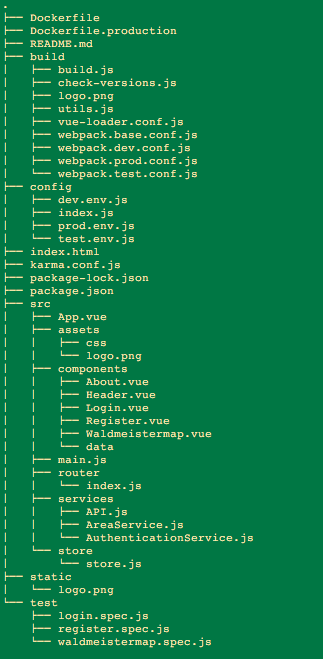
\includegraphics[width=0.6\textwidth]{client}
    \caption{Package-Struktur, Client}
    \label{fig:ps1}
\end{figure}

\begin{figure}[H]
\centering
    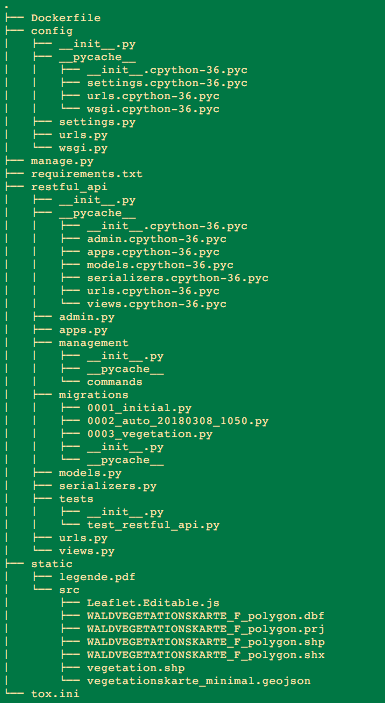
\includegraphics[width=0.6\textwidth]{backend}
    \caption{Package-Struktur, Backend}
    \label{fig:ps2}
\end{figure}

\begin{figure}[H]
\centering
    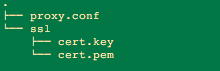
\includegraphics[width=0.4\textwidth]{nginx}
    \caption{Package-Struktur, nginx}
    \label{fig:ps4}
\end{figure}

\subsection{Sequenz-Diagramm}
Die folgenden Sequenzdiagramme geben detaillierten Einblick in den Ablauf des Registrierung - und Loginvorgangs, sowie das Laden der Public und Private Areas und deren Darstellung im Client. $\newline$

\begin{figure}[H]
\centering
    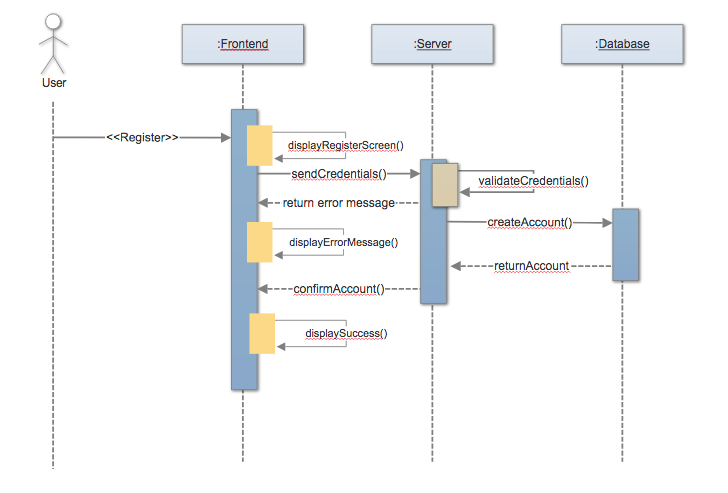
\includegraphics[width=0.8\textwidth]{Sequenz_DiagrammRegister}
    \caption{Sequenzdiagramm, Register}
    \label{fig:sd1}
\end{figure}

\begin{figure}[H]
\centering
    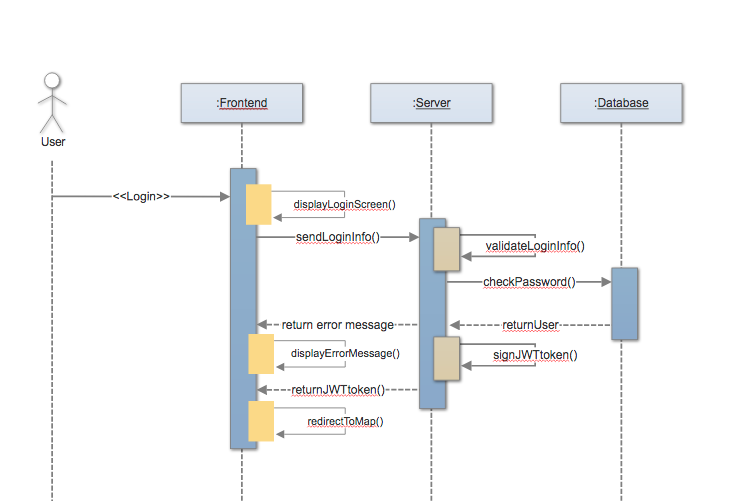
\includegraphics[width=0.8\textwidth]{Sequenz_DiagrammLogin}
    \caption{Sequenzdiagramm, Login}
    \label{fig:sd2}
\end{figure}

\begin{figure}[H]
\centering
    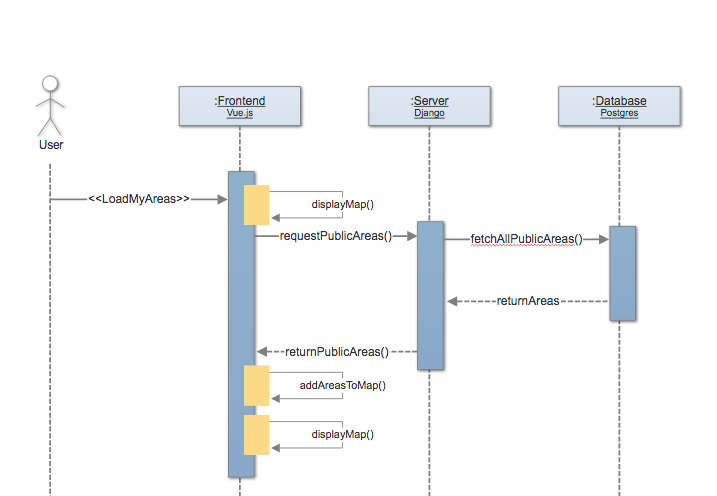
\includegraphics[width=0.8\textwidth]{Sequenz_DiagrammPublicAreas}
    \caption{Sequenzdiagramm, Public Areas}
    \label{fig:sd3}
\end{figure}

\begin{figure}[H]
\centering
    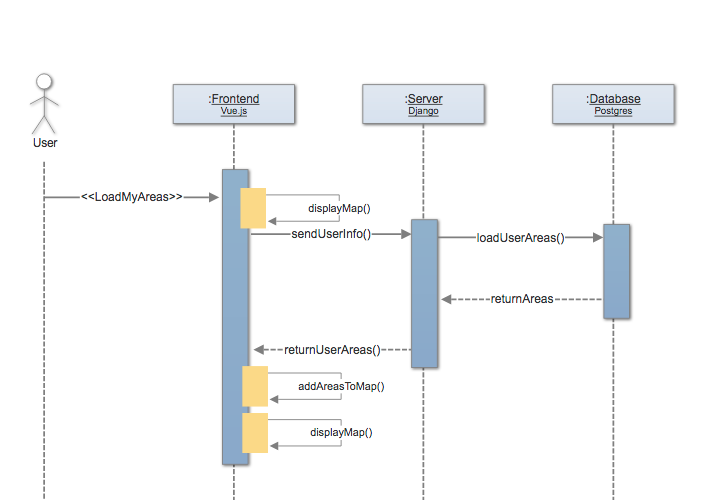
\includegraphics[width=0.8\textwidth]{Sequenz_DiagrammMyAreas}
    \caption{Sequenzdiagramm, My Areas}
    \label{fig:sd4}
\end{figure}
\pagebreak

\subsection{Komponentendiagramm}

Das Komponentendiagramm zeigt die Beziehungen zwischen verschiedenen Komponenten der Webapp. Die Waldmeistermap bezieht Daten \"uber verschiedene Interfaces welche auf der Map dargestellt oder verwendet werden.$\newline$

\begin{figure}[H]
\centering
    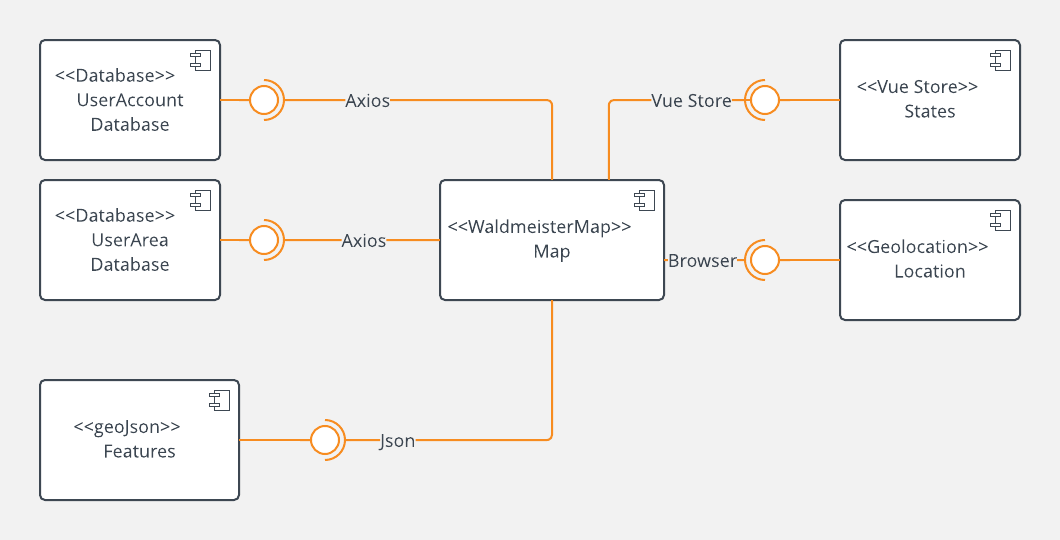
\includegraphics[width=1\textwidth]{umlwaldmeister}
    \caption{Komponentendiagramm, Waldmeister Map}
    \label{fig:kdwm}
\end{figure}


\subsection{UI Design}
\subsubsection{Mockups}
Die Mockups wurden vor der Implementation erstellt, um Screendesign und Layout klarer zu definieren, bevor es um die technische Implementation von "Waldmeister - Outdoors" ging. In den folgenden Abbildungen Eins bis Neun kann man den Arbeitsschritt Einloggen und Erstellen einer neuen Fl\"ache und eines Points of Interests (POI) sehen. Zus\"atzlich sieht der User seine eigene Location auf der Map eingetragen und hat \"uber das Menu "My Places" Zugriff auf eine Liste seiner erstellten Fl\"achen. Ein Kontextmenu gibt bei der Anzeige eines ausgew\"ahlten Objekts zus\"atzliche Informationen.

\pagebreak

\begin{figure}[H]
\centering
    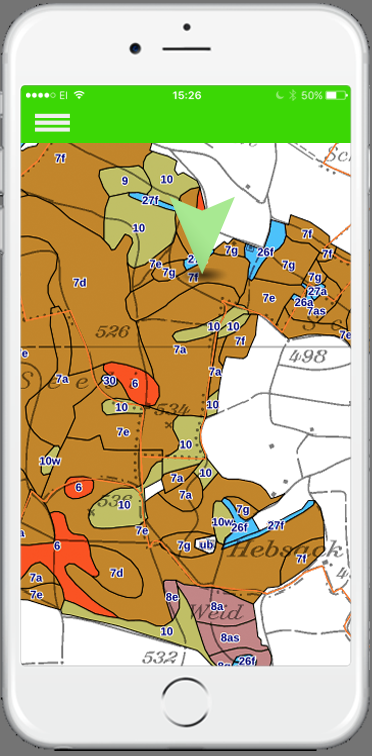
\includegraphics[width=0.29\textwidth]{mockup1-1}
    \caption{Mockup Screen 1, Anzeige des Eigenen Standorts auf der Map}
    \label{fig:mesh1}
\end{figure}

\begin{figure}[H]
\centering
    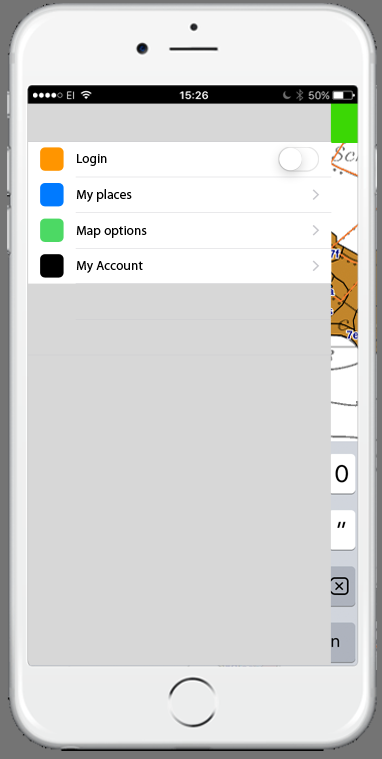
\includegraphics[width=0.29\textwidth]{mockup1-2}
    \caption{Mockup Screen 2, \"offnen des Menus, Login}
    \label{fig:mesh2}
\end{figure}

\begin{figure}[H]
\centering
    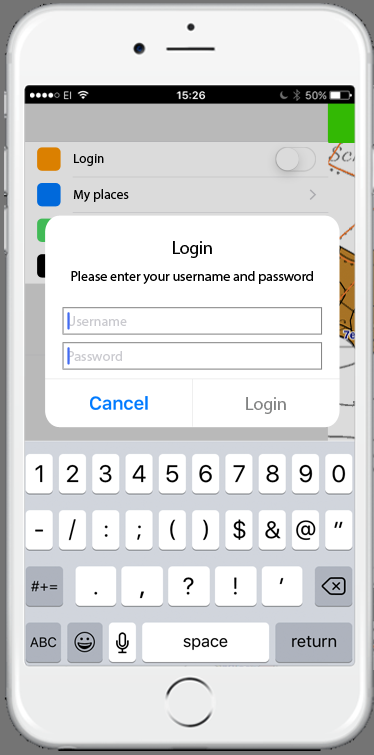
\includegraphics[width=0.29\textwidth]{mockup1-3}
    \caption{Mockup Screen 3, Eingeben der Accountdetails}
    \label{fig:mesh3}
\end{figure}

\begin{figure}[H]
\centering
    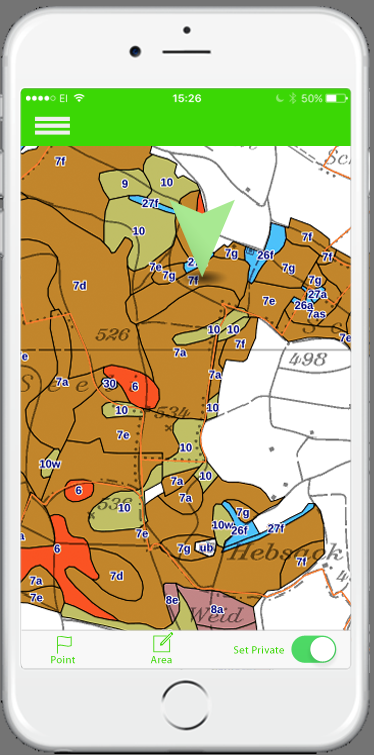
\includegraphics[width=0.29\textwidth]{mockup1-4}
    \caption{Mockup Screen 4, Map Ansicht nach dem Login}
    \label{fig:mesh4}
\end{figure}

\begin{figure}[H]
\centering
    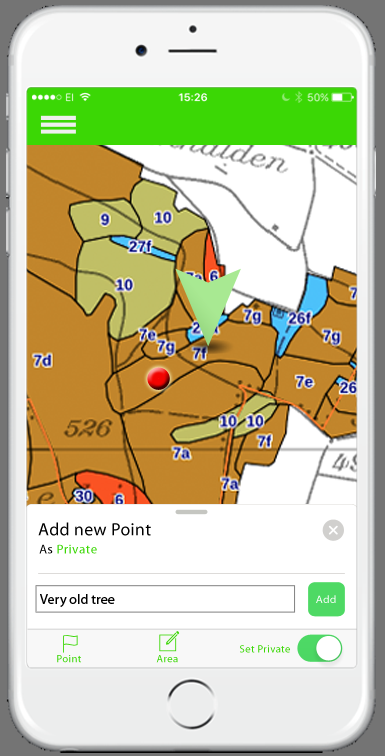
\includegraphics[width=0.29\textwidth]{mockup1-5}
    \caption{Mockup Screen 5, Erfassung eines Points of Interests}
    \label{fig:mesh5}
\end{figure}

\begin{figure}[H]
\centering
    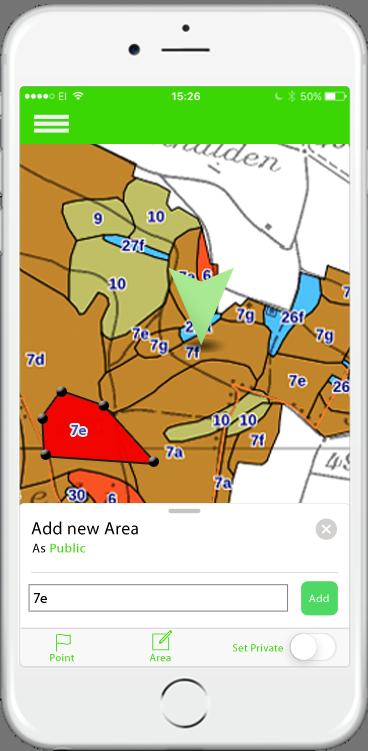
\includegraphics[width=0.29\textwidth]{mockup1-6}
    \caption{Mockup Screen 6, Erfassung einer Benutzerfl\"ache}
    \label{fig:mesh6}
\end{figure}

\begin{figure}[H]
\centering
    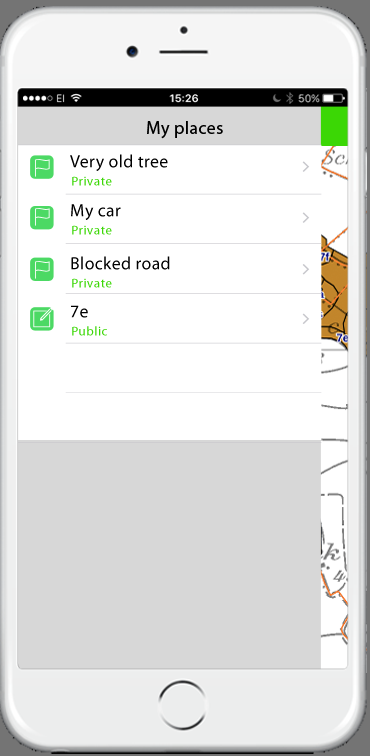
\includegraphics[width=0.29\textwidth]{mockup1-7}
    \caption{Mockup Screen 7, Auflistung aller Benutzerfl\"achen dieses Users}
    \label{fig:mesh7}
\end{figure}

\begin{figure}[H]
\centering
    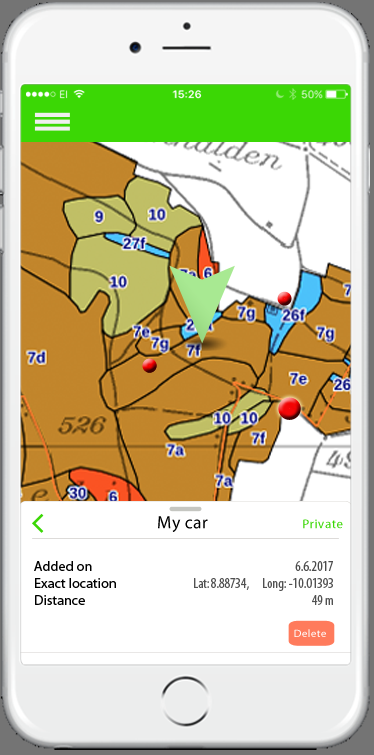
\includegraphics[width=0.29\textwidth]{mockup1-8}
    \caption{Mockup Screen 8, Detailansicht eines selektierten Points of Interests}
    \label{fig:mesh8}
\end{figure}

\begin{figure}[H]
\centering
    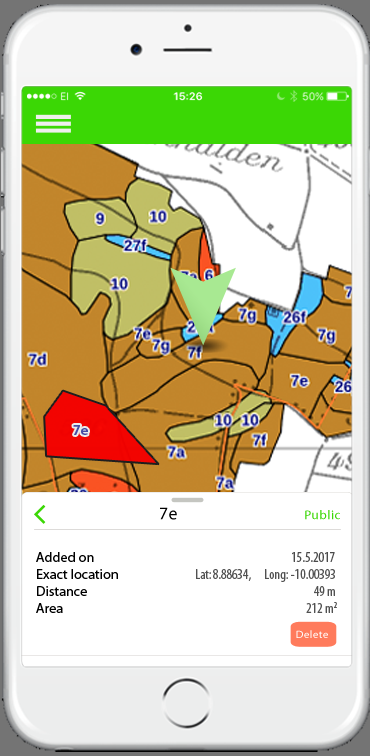
\includegraphics[width=0.29\textwidth]{mockup1-9}
    \caption{Mockup Screen 9, Detailansicht einer selektierten Benutzerfl\"ache}
    \label{fig:mesh9}
\end{figure}

\pagebreak

\section{Implementation}
\subsection{Vue Komponenten}
Die Applikation "Waldmeister - Outdoors" setzt sich aus den Komponenten Register, Login, About, der WaldmeisterMap und einem Page Header zusammen. Dar\"uber hinaus bildet die Komponente "App.vue" die Basis, um den Page Header und Router-View Komponenten zu laden. $\newline$

\subsubsection{Vue Map Komponente}
Die Komponente WaldmeisterMap ist die Vue Komponente, auf welcher die Leaflet Map und darauf die Layer Vegetationskarte (als geoJSON) und der Layer f\"ur die Benutzerfl\"achen (als Polygone) dargestellt werden. Das Leaflet Map Objekt beinhaltet auch die Kontrollbuttons, welche mit der Map assoziiert sind. Durch die Buttons 'Veg' und 'UAs' in der oberen linken Ecke der Map k\"onnen die GeoJSON bzw die Benutzerfl\"achen ein - und ausgeschaltet werden. Dadurch werden die Layer, auf welchen sich die Polygone befinden gecleart und alle erstellten Labels von der Map gel\"oscht. Bet\"atigt der User den Button noch einmal, werden sie erneut erstellt. Sie sind standardm\"assig eingeschaltet und werden daher auch erstellt, wenn das Map Objekt auf die Page gemountet wird (beim Laden der WaldmeisterMap Komponente). Damit Label und Polygone der verschiedenen Layer separat ein- und ausgeschaltet werden k\"onnen, werden sie zuerst in Gruppen unterteilt, bevor diese Gruppen auf die Map hinzugef\"ugt werden.$\newline$
Oberhalb dieser zwei Buttons befindet sich der "Add" Button, welcher es dem User erm\"oglicht, eine neue Benutzerfl\"ache auf der Map einzutragen. Er kann, w\"ahrend er im Zeichnungsmodus ist, per click event dem Polygon einen neuen Eckpunkt anh\"angen. Klickt der User w\"ahrend des Zeichnungsmodus auf den ersten erstellten Eckpunkt, schliesst sich das Polygon und der User wird per Dialogbox aufgefordert, dem erstellten Objekt die ben\"otigten Attribute zuzuweisen (label, public). Dr\"uckt er in diesem Dialog auf "Save" wird die Fl\"ache an den Server geschickt und in der Datenbank gespeichert. $\newline$

\subsubsection{Registrierung und Login}
Registrierung und Login wurden als separate Single-File-Komponenten aufgebaut, damit sie vom Vue-Router dargestellt werden k\"onnen. Sie beinhalten die Felder Username, Passwort und bei der Registrierung auch ein Email Feld, welches optional ist. Bei der erfolgreichen Registrierung wird von Djoser ein Benutzer angelegt und sein Passwort im verschl\"usselten Zustand hinterlegt. Loggt sich der Benutzer mit den korrekten Daten ein, erh\"alt er vom Server ein JWT (JSON Web Token), welches von Djoser basierend auf dem hinterlegten Accounts erstellt wird. Der Vue-Client Server hinterlegt dieses Token im Vue Store, damit es in verschiedenen Komponenten verwendet werden kann. Um sich dem Server gegen\"uber zu authentifizieren wird es bei einem Request mitgeschickt. Loggt er sich aus, wird dieses Token aus dem Store gel\"oscht. Der User kann sich erneut oder unter einem anderen Benutzernamen und Passwort einloggen. $\newline$
Bei nicht erfolgreichen Versuchen, einen Account zu erstellen oder sich einzuloggen, werden dem User diverse Fehlermeldungen angezeigt, welche Auskunft \"uber fehlerhafte Passworteingabe oder Benutzerdaten bei der Erstellung des Accounts geben. $\newline$
Nach einem erfolgreichen Login wird der User per Vue-Router auf die Komponente WaldmeisterMap weitergeleitet und alle Benutzerfl\"achen werden vom Server angefordert, auf die er Zugriff hat. Der Server liefert per REST Interface alle \"offentlichen Benutzerfl\"achen, sowie die privaten Benutzerfl\"achen, welche diesem User zugeordnet sind. \cite{djoserpack} $\newline$

\subsubsection{About}
Die Komponente About enth\"alt wichtige Informationen zu den dargestellten Daten und beinhaltet die Links zu den nativen iOS und Android Apps, unter welchen das Nachschlagewerk "Waldmeister" erh\"altlich ist. Unterhalb des dargestellten Logos befinden sich ausserdem Informationen zum Projekt und den Rahmenbedingungen, unter welchen es erstellt wurde. $\newline$
Hier wird auch dem Kanton Z\"urich gedankt f\"ur die Nutzungsrechte der Daten "Vegetationskundliche Kartierung der Waldfl\"achen im Kanton Z\"urich".

\begin{figure}[H]
\centering
    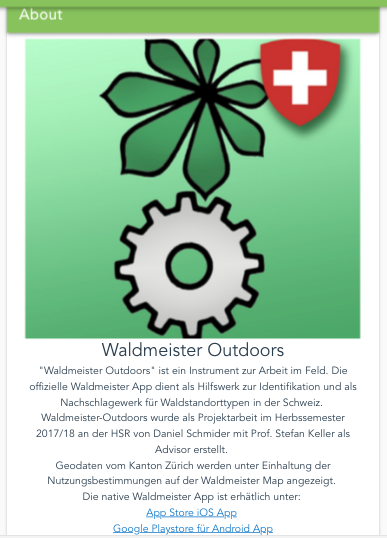
\includegraphics[width=0.5\textwidth]{aboutscreen}
    \caption{About in der Waldmeister-Outoors Webapp}
    \label{fig:aboutscreen}
\end{figure}

\subsection{Frontend Design}
Das User Interface wurde gr\"osstenteils mit Vuetify realisiert, welches die \"aussere Erscheinung der Komponenten Header, Registrierung, Login, About, etc... bestimmt. Es wurde auf das Farbschema der existierenden Waldmeister App angepasst und eignet sich, um eine Webapp responsive zu gestalten, damit sie auf mobilen Ger\"aten ebenfalls korrekt dargestellt wird. $\newline$
Weitere Teile, vor allem Elemente welche sich auf der Leaflet Map befinden, wurden mit CSS Styling aufgewertet. Der GeoJSON Layer, welcher die Fl\"achen der Waldstandorte anzeigt, wird durch CSS dazu verwendet jedes Polygon auf diesem Layer aufgrund von einem Property des Polygons einzuf\"arben. Dieses Property ist die EK72 Kennzahl, bzw. K\"urzel. Jedem dieser K\"urzel kann eine bestimmte Farbe zugewiesen werden, welche als hexadezimale, 6-stellige Zahl im Code repr\"asentiert wird. Jedes Polygon erh\"alt dar\"uber hinaus auch ein Label, welches dieses K\"urzel ebenfalls darstellt. Diese Property Label haben eine weisse Schrift, sind nicht transparent und haben einen 2 Pixel weiten Schatten, damit sie sich von der Hintergrundfarbe abheben.$\newline$

\begin{figure}[H]
\centering
    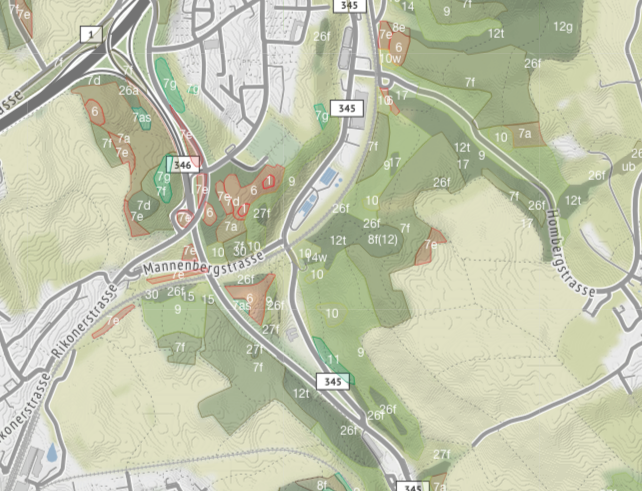
\includegraphics[width=1\textwidth]{propertylabel}
    \caption{Einf\"arbung von GeoJSON Fl\"achen und Darstellung von PropertyLabels}
    \label{fig:propertylabel}
\end{figure}

$\newline$
Benutzerfl\"achen werden blau dargestellt und haben ein gef\"arbtes Label, damit sie sich von den Fl\"achen des geoJSON Layers unterscheiden. Private Fl\"achen haben ein gelbes Label, \"offentliche sind gr\"un. Dar\"uber hinaus haben sie eine breitere Outline als Fl\"achen des GeoJSON Layers.

\begin{figure}[H]
\centering
    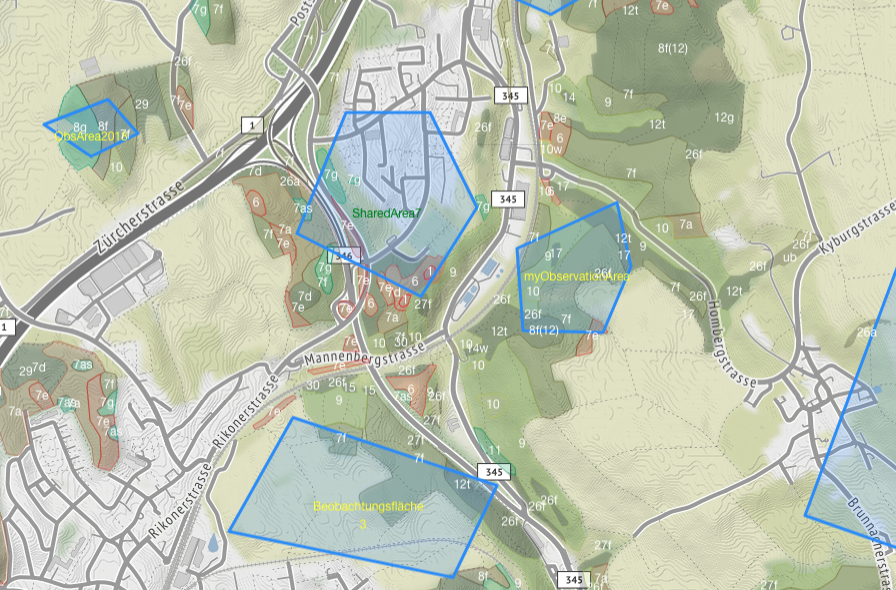
\includegraphics[width=1\textwidth]{userareas}
    \caption{Benutzerfl\"achen mit Labels}
    \label{fig:userareslabels}
\end{figure}
$\newline$
Die Geolocation wird als blauer "Circle" dargestellt. Die Gr\"osse des Kreises repr\"asentiert die Genauigkeit der Berechnung der Geolocation in Metern. $\newline$

\begin{figure}[H]
\centering
    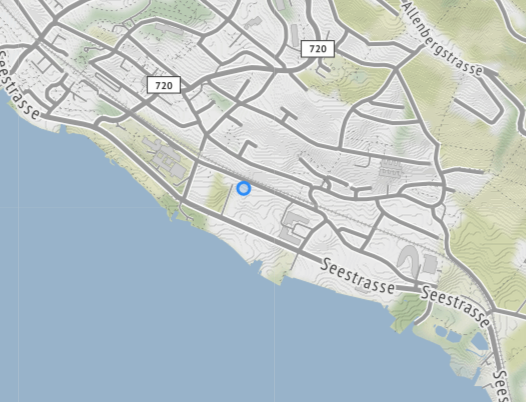
\includegraphics[width=1\textwidth]{geolocation}
    \caption{Geolocation auf der Map als Circle sichtbar}
    \label{fig:geoloc1}
\end{figure}
$\newline$
Die Buttons welche den Zeichungsmodus starten oder beenden oder Ebenen ein- und ausblenden sind in der oberen linken Ecke, unterhalb der Zoombuttons vertikal aufgereiht. Der Zeichnungsbutton ist mit "Add" beschriftet und wechselt auf "Edit" solange der Zeichnugsmodus aktiviert ist. Die Buttons zum Ein- und Ausblenden von Ebenen sind mit "Veg" und "Areas" beschriftet, haben aber l\"angere Tooltips, welche die Funktion genauer beschreiben. $\newline$
$\newline$
Die "Save" Dialogbox wird nur angezeigt, wenn eine gezeichnete Fl\"ache durch einen Klick auf den ersten gezeichneten Eckpunkt geschlossen wird. Durch den "Save" Button innerhalb der Dialogbox werden die Werte f\"ur Label und Public \"ubernommen und das gezeichnete Polygon wird per REST Schnittstelle an den Server geschickt, damit es in der Datenbank gespeichert wird.

\subsection{Geolocation}
Damit der eigene Standort auf der Map eingetragen oder die Map auf diesen Punkt zentriert werden kann, muss die Webapp HTTPS Secure (Https) verwenden, da die meisten Webbrowser es nicht zulassen, den Standort eines Users zu ermitteln, ohne dass die Verbindung gesch\"utzt ist. Um den Transport Layer zu verschl\"usseln wird ein self-signed Zertifikat verwendet, welches auf dem Vue-Client hinterlegt wird. Es besteht aus einer cert.pem und einer key.pem file. Browser werden zwar eine Warnung f\"ur solche Zertifikate einblenden, k\"onnen aber eine verschl\"usselte Verbindung aufbauen, nachdem sie zugelassen wird. $\newline$
Danach k\"onnen die Funktionen von HTML 5, z.B navigator.geolocation.getCurrentPosition() verwendet werden, welche einen Punkt mit Latitude und Longitude zur\"uckgibt. Zu diesem Punkt gibt es zus\"atzlich einen Accuracy Wert, welcher die Genauigkeit der Berechnung in Metern angibt.

\subsection{API}
Diese Anfragen werden vom Client \"uber eine Axios API abgesetzt. Nach der Initialisierung des Axios Services wird eine Base Url bestimmt, welche auf das Backend im Django Server zielt. Mit jedem Request, welches \"uber diesen Service ausgef\"uhrt wird, wird auch das im Store hinterlegte JWT Token mitgeschickt, sofern es existiert. Falls nicht, wird der User als nicht autorisiert identifiziert.
Neben der Authentication Service, welcher die Methoden Register und Login ausl\"osen kann, besteht der AreaService, welcher per getAreas und postAreas Benutzerfl\"achen vom Server anfordern oder an den Server schicken kann, damit sie in der Datenbank erstellt werden. Die Erstellung von neuen Fl\"achen ist jedoch nur m\"oglich, wenn der User sich eingeloggt hat.$\newline$
Abh\"angig vom Request f\"ugt Axios Service eine URL-Endung an die Basisurl an, damit Django per Routingsystem erfassen kann, um welche Art Request es sich handelt. Post Requests innerhalb des AuthenticationServices kommunizieren mit den Djoser definierten URL-Endungen /auth/users/create (um beispielsweise einen neuen Benutzer zu registieren). Diesem Post Request werden die credentials mitgeschickt, welche vom User im Client eingegeben wurden. Dieses credentials-Objekt besteht aus username, password und email. Sie werden als JSON Objekt an den Django Server geschickt.$\newline$
Neben dem AuthenticationService regelt der AreaService per get und post requests \"uber die URL-Endungen '/api/areas/' Requests bez\"uglich Benutzerfl\"achen.
Axios kommuniziert mit dem Server \"uber eine REST-Schnittstelle. Benutzerfl\"achen werden per Get-Request an den Client \"ubertragen, neu erfasste Benutzerfl\"achen werden \"uber einen Post-Request als JSON Objekte an den Server \"ubertragen. Django deserialisiert diese JSON Objekte und speichert sie anschliessend in der PostgreSQL Datenbank. $\newline$

\subsubsection{API Dokumentation, Swagger}
Die API Dokumentation wurde mit dem Python Package Swagger implementiert und kann \"uber die URL WaldmeisterMap/swagger/ aufgerufen werden. Sie gibt Information \"uber alle verf\"ugbaren API Requests und deren Funktionen. Die API gliedert sich in die URLs der Benutzeraccount Erstellung (WaldmeisterMap/auth/) und die API Requests welche f\"ur die Erstellung von Benutzerfl\"achen zust\"andig sind (WaldmeisterMap/api/areas/). $\newline$
Benutzeraccounts werden vom Python Package Djoser erstellt. Dieses Package beinhaltet unter anderem die URL /WaldmeisterMap/auth/users/create/, welches mit den Attributen "email, username, password" einen neuen User in der Datenbank registriert. Nach der erfolgreichen Registrierung kann \"uber die URL /WaldmeisterMap/auth/token/create/ ein JWT Token vom Server angefordert werden. Dieser Request hat die Attribute "username, password". Stimmen die Werte mit einem existierenden Account in der Datenbank \"uberein, wird dem Client als Antwort ein JWT Token geliefert, welches der Client mit darauffolgenden Requests mitschicken kann, damit der Server den User mit einem registrierten User in der Datenbank verkn\"upfen kann. JWT Tokens laufen nach einer bestimmten Zeit ab oder z.B. wenn der Django Server sich neu initialisiert. Ein JWT Token kann \"uber die URL /WaldmeisterMap/auth/jwt/refresh/ erneuert werden, in dem das existierende Token im POST Request mitgeschickt wird.
$\newline$
Benutzerfl\"achen werden \"uber die URL /WaldmeisterMap/api/areas/ als GET Request abgefragt. Der Request liefert anhand vom eingeloggten oder nicht eingeloggten Usern \"offentliche Fl\"achen, bzw. auch die privaten Fl\"achen des authentifizierten Users, welche unter seinem Account in der Datenbank gespeichert sind. \"Uber die gleiche URL kann mit einem POST Request eine neue Benutzerfl\"ache in der Datenbank erstellt werden. \"Uber die URLs /WaldmeisterMap/api/areas/id kann auf eine spezifische, existierende Benutzerfl\"ache die Requests GET, DELETE, PATCH und PUT ausgef\"uhrt werden, um diese bestehende Benutzerfl\"ache zu bearbeiten, bzw. zu l\"oschen. Sie wird \"uber die URL-Endung "id" referenziert.$\newline$
\"Uber die API kann auch abgefragt werden, ob sich die ermittelte GPS Position des Ger\"ats zu diesem Zeitpunkt gerade innerhalb eines Waldstandorts befindet, welcher in der Datenbank eingetragen ist.

\begin{figure}[H]
\centering
    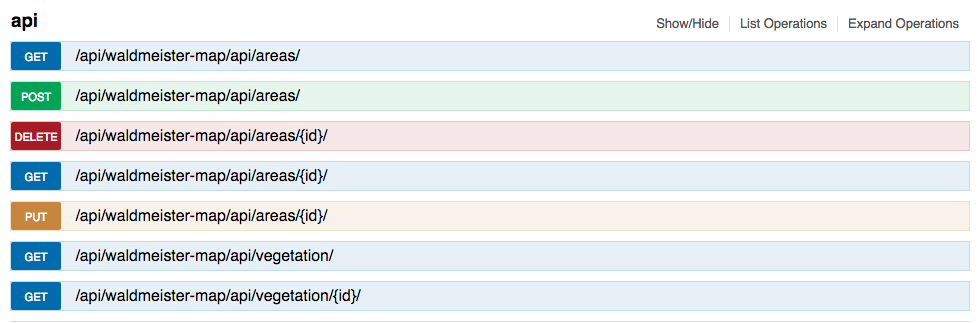
\includegraphics[width=1\textwidth]{swagger1}
    \caption{Swagger API Authorization}
    \label{fig:swagger1}
\end{figure}

\begin{figure}[H]
\centering
    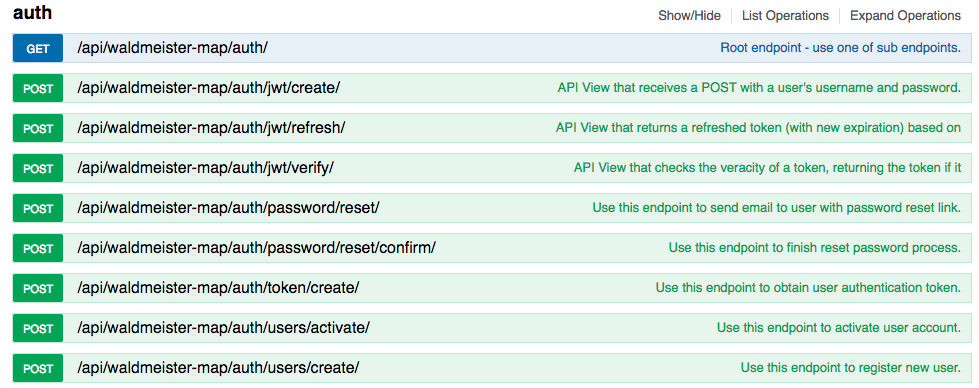
\includegraphics[width=1\textwidth]{swagger2}
    \caption{Swagger API UserAreas}
    \label{fig:swagger2}
\end{figure}

\begin{figure}[H]
\centering
    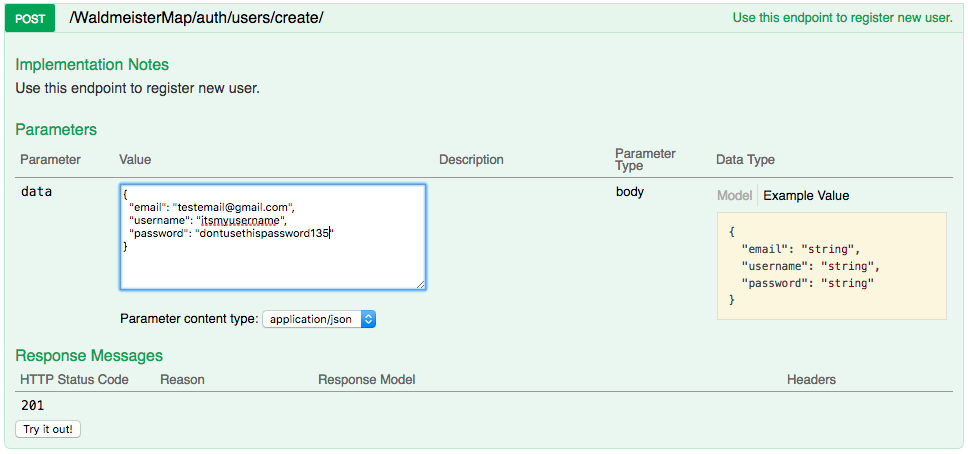
\includegraphics[width=1\textwidth]{swaggerdetails}
    \caption{Swagger API user create Details}
    \label{fig:swagger3}
\end{figure}

\subsection{Database}
Die Benutzerfl\"achen und Vegetationsfl\"achen werden von Django durch ein Django-Dabatase-Model beschrieben und haben die Attribute "label, public, polygon und creator".   $\newline$
"Label" ist ein Feld, welches aus Charakteren und Ziffern besteht. $\newline$
Das Feld 'public' ist ein Boolean Wert, welcher bestimmt, ob eine Fl\"ache \"offentlich oder privat gehandhabt wird. $\newline$
'polygon' beinhaltet die Geometrie, die Art der Fl\"ache und das Format, in welcher sie in der Datenbank gespeichert wird. Die Geometrie ist Teil des polygon field und beinhaltet ein Array, welches Punkte in Longitude / Latitude Paaren enth\"alt, welche die Eckpunkte des Polygons beschreiben. Dies k\"onnen beliebig viele sein und im Falle eines Multipolygons kann dieses Feld auch mehrere Arrays beinhalten, welche wiederum ein einzelnes Polygon beschreiben. \"Uberschneiden sich mehrere Polygone entstehen "Inseln", welche nicht zu der Fl\"ache des Multipolygons geh\"oren.$\newline$
Also Koordinatensystem wird das System WGS84 mit der SRID 4326 verwendet. \cite{srid}  $\newline$
Vegetationsfl\"achen werden in der Datenbank als Multipolygone und einem K\"urzel nach EK72 in der Form von Zahlen und Charakteren gespeichert.
 $\newline$
 Die Django Datenbank Modells befinden sich im Ordner "restful_api" des backends in der Datei models.py

\subsubsection{Database, PostgreSQL}
F\"ur die Kommunikation zwischen Django und PostgreSQL wird das Python Package Psycopg2 verwendet. Dieses Package ist der verbreitetste PostgreSQL Datenbank Adaptor f\"ur die Python Programmiersprache. $\newline$
Als Datenbank wird PostgreSQL 10 verwendet. Die Datenbank Verbindungsdetails sind in der Python settings.py Datei eingetragen. Waldmeister-Outdoors wird versuchen, auf eine lokale Datenbank mit dem Namen 'dschwaldmeister' zuzugreifen. Username ist postgres und der Port ist standardm\"assig auf 5432 gesetzt. Die "Engine" wurde ebenfalls auf 'django.contrib.gis.db.backends.postgis' ge\"andert, da postgis auf der Datenbank verwendet wird und als Extension installiert werden muss. Mit psql \"uber die Konsole oder PGAdmin4 k\"onnen auf die lokale PostgreSQL Datenbank zugegriffen, Daten manuell gel\"oscht oder eingetragen werden.

\subsection{Kartenmaterial}
Die Daten f\"ur den Vegetationslayer wurden vom Kanton Z\"urich (maps.zh.ch) \"ubernommen und werden von der Webapp als Polygone auf der Leaflet Map dargestellt. Sie werden vom Django Backend nach erfolgreichem Starten des Servers in die Datenbank geladen. 

\pagebreak
\section{Tests}
Testgetriebene Entwicklung (TDD) ist eine Methode zur Softwareentwicklung, welche oft bei der agilen Entwicklung von Computerprogrammen eingesetzt wird. Bei TDD erstellt der Programmierer Software-Tests, um das korrekte Verhalten von Softwarekomponenten zu planen und zu \"uberpr\"ufen. Unit Tests (auch als Unittest oder als Komponententest bezeichnet), werden verwendet um die funktionalen Einzelteile eines Softwareprojekts zu pr\"ufen. 

\subsection{Tests in Django}
Test f\"ur das Django wurden mit dem Standard Django Modul "unittest" erstellt. Es wurden Tests zu Login, Registrierung und Erstellung von Benutzerfl\"achen erstellt. Es werden unvollst\"andige, fehlerhafte und nicht authorisierte Requests (zum Beispiel ohne sich einzuloggen) getestet. HTTP-Statuscode geben Auskunft \"uber die korrekte Ausf\"uhrung oder fehlerhaftes Verhalten des Servers. Sie werden verglichen mit zu erwartenden Codes und bestimmen auf diese Weise ob der Test bestanden oder gescheitert ist. $\newline$
$\newline$
Es wird getestet ob Email und Passwort vorhanden ist und ob die Anforderungen an die Werte erf\"ullt sind, ob Accounts und JWTs erstellt werden k\"onnen und ob Benutzerfl\"achen vom System korrekt erstellt werden. $\newline$
Die Tests k\"onnen mit dem Befehl "python3 manage.py test WaldmeisterMap" ausgel\"ost werden. Fehlerhafte Test werden von Django gemeldet.

\subsection{Tests in Karma}
Tests f\"ur Vue.JS wurden mit dem Test Runner Karma und dem Testframework Jasmine erstellt . Sie k\"onnen \"uber den Befehl "npm run test" ausgef\"uhrt werden, aus dem "client" folder des Vue-Servers. $\newline$
Getestet werden Komponenten und deren Inhalt, welche von VueJS verwendet werden. $\newline$
Damit Jasmin die Tests ausf\"uhren kann, muss der Code von Webpack zuerst kompiliert werden. Danach wird er in einer Browserumgebung (z.B Chrome oder Firefox) ausgef\"uhrt und das Testframework sammelt die zu testenden Werte und Verhalten. Es vergleicht diese mit gegebenen Werten und Zust\"anden, welche vom Programmierer erwartet werden. Stimmen sie \"uberein, ist der Test bestanden. Stimmen sie nicht \"uberein, ist der Test gescheitert und Jasmine meldet einen Fehler.

\subsection{Linter}
Linter werden als Werkzeuge eingesetzt, welche w\"ahrend der Entwicklung eine statische von Analyse Quellcode ausf\"uhren. $\newline$
Beim Linten von Code wird dieser auf gewisse Qualit\"atskontrollen oder Linting-Regeln gepr\"uft. Linter helfen Enwicklern, Code auf h\"oherem Qualit\"atsstandard zu schreiben, reduzieren die Anzahl Bugs, Syntax-Errors oder schlechte Formatierungen welche im Source-Code vorkommen. Dadurch wird auch die Lesbarkeit und Wartbarkeit des Codes erh\"oht. Vor allem bei Teamarbeiten ist das Einsetzen und Durchsetzen von Styleguides sehr wichtig. Durch das Einsetzen von Lintern sparen Entwickler Zeit und Code-Reviews k\"onnen schneller durchgef\"uhrt werden.

\subsubsection{Eslint}
Eslint ist ein Code-Linting Tool f\"ur JavaScript, welches daf\"ur eingesetzt wird gewisse Regeln und Styleguides w\"ahrend der Entwicklung des Projekts zu \"uberpr\"ufen. Eslint (in Kombination mit einem Texteditor wie Sublime), macht auf Codestellen aufmerksam, welche nicht den Konfigurationen entsprechen. Eingesetzt wurde der AirBnB Styleguide. Das Frontend, Entwickelt mit Vue.JS ist mit JavaScript erstellt. Daher kann das gesamte Frontend mit ESLint gelintet werden.

\subsubsection{Flake8}
Flake8 ist Linter f\"ur Python Projekte, welches daf\"ur eingesetzt wird Code-Guidelines f\"ur Python Quellcode einzuhalten. Fehler und Warnungen werden bereits bei der Erstellung des Sourcecodes im Editor angezeigt.

\subsection{Continuous Integration}
\subsubsection{Travis}
Um Continuous mit automated build und testing zu realisieren, wurde Travis verwendet. Die Software Travis CI wurde 2011 in Berlin erstellt und 2013 ver\"offentlicht. Auf der Website travis-ci.org wird das Repo, welches auf Github gehostet wird, verkn\"upft. Jedes mal wenn auf das remote Repo (auf GitHub) gepusht wird, f\"uhrt Travis die config in Form einer .yml Datei aus, welche im root Ordner des Repos hinterlegt ist. Sie installiert alle Programme und Dependancies auf einer Linux Maschine, buildet das Projekt und testet ob der Build in der aktuellen Version funktioniert. Es entsteht eine Version History mit dazugeh\"orender config. Travis meldet, ob der Build und die Tests erfolgreich durchgef\"uhrt werden konnten. Dies geschieht auch auf separaten Branches des Projekts. $\newline$
Nachdem das Projekt erfolgreich gebuildet worden ist, werden die erstellten Dockerimages von Travis als auf DockerHub hochgeladen. Images, welche auf DockerHub gehosted werden k\"onnen sp\"ater von Docker gepullt werden, zum Beispiel wenn das Projekt auf einem Server deployt wird.

\begin{figure}[H]
    \centering
    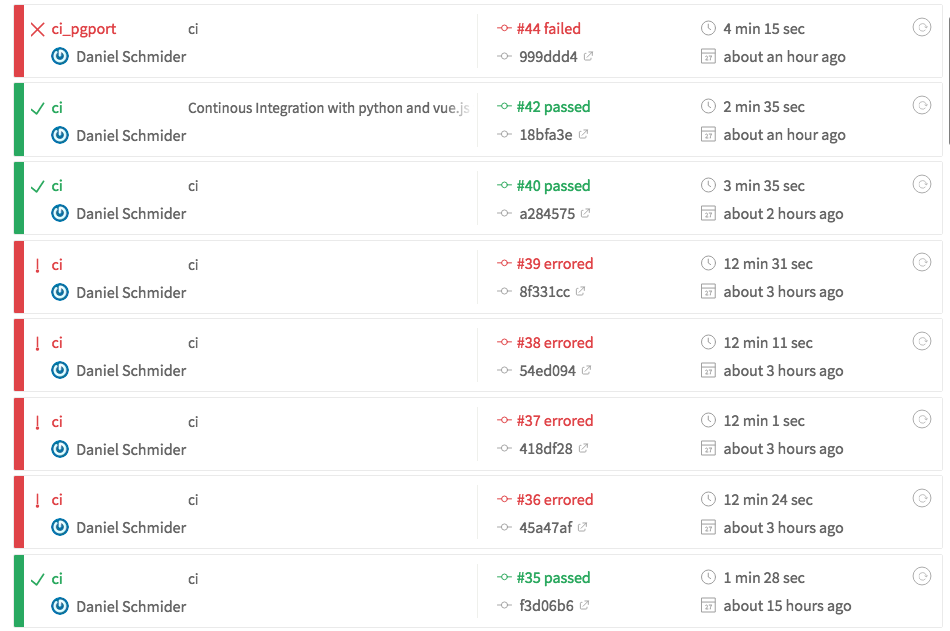
\includegraphics[width=1\textwidth]{travisv}
    \caption{TravisCI Version History}
    \label{fig:t1}
\end{figure}

\begin{figure}[H]
    \centering
    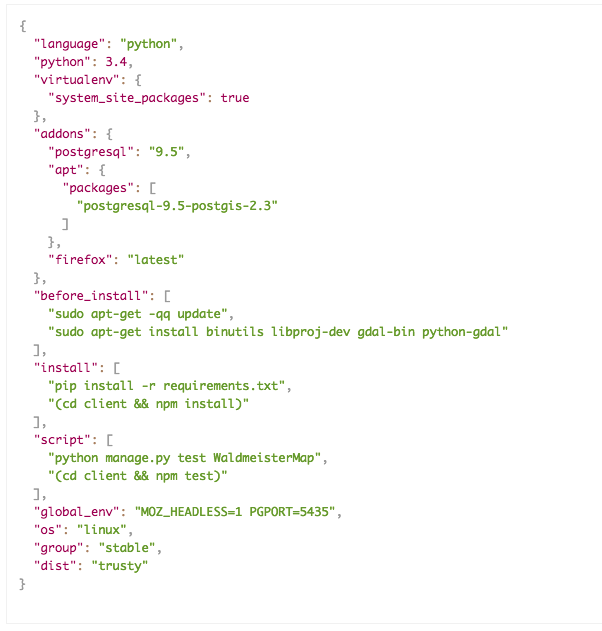
\includegraphics[width=1\textwidth]{travisc}
    \caption{Travis config .yaml, Version #45}
    \label{fig:t2}
\end{figure}

\begin{figure}[H]
    \centering
    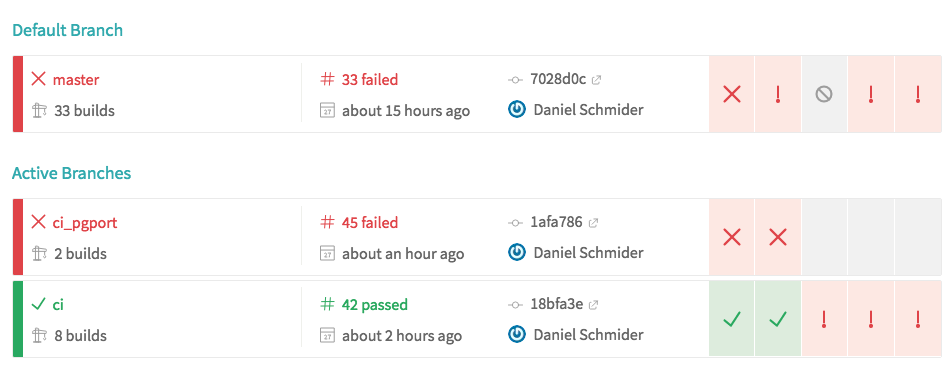
\includegraphics[width=1\textwidth]{travisb}
    \caption{Travis branches}
    \label{fig:t3}
\end{figure}

\pagebreak
\section{Manuelle Tests}
\subsection{User-Szenario}
Das User-Szenario ist ein m\"oglicher Interaktionsablauf eines Users, welcher die Webapp "Waldmeister-Outdoors" verwendet. Es ist in die verschiedenen Schritte eingeteilt, welcher der User durchf\"uhrt. $\newline$
$\newline$
1. Aufrufen der URL $\newline$
2. Pan & Zoom der Map auf einen beliebigen Bereich $\newline$
3. Aufruf der "About" Seite $\newline$
4. \"Offnen der Map-Legende in einem separaten Tab $\newline$
5. Registrierung eines neuen Users, Eingabe von Benutzernamen und Passwort $\newline$
6. Login mit dem neu erstellten Benutzer $\newline$
7. Erstellung einer neuen privaten Benutzerfl\"ache $\newline$
8. Updaten der gerade erstellten Benutzerfl\"ache $\newline$
9. Erstellen einer neuen \"offentlicher Benutzerfl\"ache $\newline$
10. Erstellen einer zweiten \"offnentlicher Benutzerfl\"ache $\newline$
11. L\"oschen einer \"offentlicher Benutzerfl\"ache $\newline$
12. Ausloggen des Benutzers $\newline$
13. Aufruf der Map im ausgeloggtem Zustand $\newline$
14. Anzeige der \"offentlichen Benutzerfl\"ache $\newline$
15. Registrierung eines zweiten Benutzers $\newline$
16. Einloggen des zweiten Benutzers $\newline$
17. L\"oschungsversuch einer \"offentlichen Benutzerfl\"ache, welche vom ersten Nutzer erstellt wurde $\newline$
18. Erstellen einer \"offentlichen Benutzerfl\"ache $\newline$
19. Updaten der erstellen Benutzerfl\"ache, wechseln des Labels und \"offentlich auf privat $\newline$

\subsection{Testf\"alle}
Testfall A: $\newline$
Aufruf der URL $\newline$
Erwartet: Laden der Webapp$\newline$
Erf\"ullt: Ja/Nein$\newline$
$\newline$
Testfall B:$\newline$
Pan und Zoom der Map$\newline$
Erwartet: Kartenausschnitt bewegt sich durch drag & drop, zoomen durch Mousewheel (Gesture bei mobilen Ger\"aten) oder Zoom Buttons
Erf\"ullt: Ja/Nein$\newline$
$\newline$
Testfall C:$\newline$
Registrierung und Login$\newline$
Erwartet: Registrierung durch Eingabe eines noch nicht verwendeten Usernamens und Passworts, Login durch die selben Informationen
Erf\"ullt: Ja/Nein$\newline$
$\newline$
Testfall D:$\newline$
Erstellen von Benutzerfl\"achen$\newline$
Erwartet: Erstellung einer beliebigen Benutzerfl\"ache durch aktivieren des "Add" buttons. Eckpunkte des Polygons bezeichnen. Durch erneute auswahl eines bereits existierenden Eckpunkts wird die Fl\"ache geschlossen und Dialogbox zum speichern der Fl\"ache \"offnet sich.
Erf\"ullt: Ja/Nein$\newline$
$\newline$
Testfall D:$\newline$
Updaten einer existierenden Benutzerfl\"ache$\newline$
Erwartet: Updaten einer exisierenden Benutzerfl\"ache, in dem im eingeloggtem Zustand eine eigene Benutzerfl\"ache (\"offentlich oder privat) angew\"ahlt wird. \"Andern der Eckpunkte der Benutzerfl\"ache durch drag & drop. Klick der Schaltfl\"ache "Upd" \"offnet Dialogbox "Update". User kann der Fl\"ache ein neues Label geben oder Schaltfl\"ache privat / \"offentlich wechseln. Durch klick auf "Update" wird die Fl\"ache und das Label neu gezeichnet.
Erf\"ullt: Ja/Nein$\newline$
$\newline$

\subsection{Reproduktion und Auswertung}
Falls ein Testfall von einem Testuser nicht korrekt ausgef\"uhrt wurde, sollte der Zustand welcher nach dem Testfall vorliegt reproduziert werden, in dem alle Interaktionen, welche der User tats\"achlich ausgef\"uhrt hat, festgehalten werden. Falls es sich um einem Bug haltet sollte ein issue erfasst werden. Falls der Fehler nicht durch einen Bug verursacht wurde, sollte es als negative User Experience festgehalten werden. F\"uhrt der Testfall in vielen F\"allen zu einer negativen User Experience, sollte das Applikationsdesign ver\"andert werden, Buttons, Labels oder Hints angepasst werden.

\pagebreak
\section{Resultate und Weiterentwicklung}
\subsection{Resultate}
User k\"onnen mittels der Webapp Waldmeister-Outdoors die Vegetationskundliche Karte erforschen und diese mit Ihrem momentanen Standort abgleichen. User k\"onnen, nachdem sie sich registriert haben, private und \"offentliche Benutzerfl\"achen erfassen und sie auf einem zentralen Server hinterlegen. Dies k\"onnen sowohl bisher nicht erfasste Waldstandorte, oder pers\"onliche Orte und Fl\"achen beschreiben, welche f\"ur Sie im Arbeitsalltag relevant sind. Solche Benutzerfl\"achen k\"onnen sie zwischen verschiedenen Ger\"aten (Im Feld und im B\"uro) abrufen oder mit anderen Personen teilen, sobald sie die Fl\"ache \"offentlich und daher von allen Usern abrufbar machen. $\newline$
Ebenfalls wurde erreicht die Geolocation auf der Karte darzustellen. Dies ist im Arbeitsalltag eine grosse Hilfe, und dient zur schnellen Orientierung und Auffindung von bestimmten eingetragenen Fl\"achen und Orten im Feld. $\newline$
Die Webapp kann sowohl auf Desktop Browsern wie von mobilen Ger\"aten verwendet werden und verh\"alt sich dank Vue.js responsive auf eine \"Anderung des Viewports, zum Beispiel wenn der Screen eines mobilen Ger\"ats w\"ahrend der Verwendung gedreht wird. $\newline$
Der Vegetationslayer und Benutzerfl\"achen-Layer und deren Label k\"onnen ein - und ausgeblendet werden, was zur \"Ubersicht beitragen kann. $\newline$
Alle Benutzeraccounts und deren Fl\"achen sind im Django Backend ersichtlich und k\"onnen als Superuser ver\"andert oder gel\"oscht werden. Wird ein Benutzer aus der Datenbank gel\"oscht, werden alle von ihm erstellten Benutzerfl\"achen ebenfalls automatisch gel\"oscht. Alle Passw\"orter von Benutzeraccounts werden verschl\"usselt in der Datenbank gespeichert. $\newline$
Zur automatischen Bestimmung des Ortabh\"angigen Waldstandorttyps wurde eine separate API entwickelt. Der Client schickt die Koordinaten an denen er sich befindet als Argumente im API Request mit, und erh\"alt vom Backend eine Response, welche beinhaltet ob an diesem Ort ein Waldstandort eingetragen ist. Der Server berechnet dies anhand der Geometrien (Polygone) des Vegetationslayers. Befindet sich der Punkt innerhalb eines Polygons, wird der Waldstandortstyp zur\"uck an den Client geschickt. Dies funktioniert auch, wenn der User sich ausserhalb der sichtbaren Map befindet, da diese Berechnung auf dem ganzen Datensatz des Vegetationslayers ausgef\"uhrt wird, nicht nur auf den Waldfl\"achen welche momentan auf dem Kartenausschnitt des Frontends angezeigt werden.

\subsection{M\"oglichkeiten der Weiterentwicklung}
\subsubsection{Vegetationsfl\"achen per API Requests}
Es wird noch ein statisches GeoJSON verwendet, welches die Vegetationsfl\"achen beinhaltet, welche auf der Map zu jedem Zeitpunkt dargestellt werden. Dies beschr\"ankt sich nicht auf dem momentanen Kartenausschnitt und f\"uhrt zu einer erh\"ohten Ladezeit beim Aufruf der Webseite, da das JSON (ca. 1mb gross) als statische Datei an den Client geschickt wird. Besonders f\"ur mobile Ger\"ate ist es sinnvoll, dies dynamisch zu gestalten und nur die ben\"otigten Vegetationsfl\"achen des Kartenausschnitts per API-Request an den Client zu schicken.

\subsubsection{Auflistung der Benutzerfl\"achen}
Um die Lokalisierung von bereits erstellten Benutzerfl\"achen zu erleichtern, w\"are es von Vorteil, diese in einer geordneten Liste darzustellen, z.B. in alphabetischer Reihenfolge oder nach ihrem Erstellungsdatum. Klickt der User auf eine dieser Listeneintr\"age, w\"urde die Map auf die Lage dieser Fl\"ache fokussieren. $\newline$
Eine solche Auflistung w\"are als aufklappbares Menu denkbar, welches sich \"uber einen Button im Header der Applikation auf - und zuklappen l\"asst.

\subsubsection{Plus Codes}
Plus Codes k\"onnen verwendet werden, um Koordinaten in eine Zeichenfolge umzuwandeln. Es wird dazu verwendet, einem Ort auf der Welt gewissermassen eine Adresse zu geben, \"ahnlich wie eine Strassenadresse. Statt einen Punkt in geografische Breite und L\"ange zu beschreiben, ist die Zeichenfolge lediglich 7 oder 11 stellig (Eine Stelle ist dabei immer das namengebende + oder - Zeichen, welches die Zeichenkette auch von internationalen Postleitzahlen abhebt). Je nachdem, ob der Code einen Ort lokal oder weltweit beschreibt, k\"onnen die vier ersten Ziffern weggelassen werden, da es ersichtlich ist, um welche weltweite Region (ca. 100 Kilometern) es sich handelt. Dies funktioniert \"ahnlich wie eine Vorwahl bei Telefonnummern, welche regional nicht ben\"otigt wird. Die vollst\"andige Zeichenfolge beschreibt einen Ort auf dem Planeten mit einer Genauigkeit von 14 auf 14 Metern. Es kann jedoch ein weiteres Zeichen angeh\"angt werden, um die Genaugkeit auf drei auf drei Meter zu erh\"ohen. Plus Codes beschreiben immer eine Fl\"ache, keinen genauen Punkt.$\newline$
Plus Codes k\"onnen offline en- oder dekodiert werden.  \cite{PluCo} $\newline$
Sie basieren auf Open Location Code (OLC), ein open-source Projekt, welches von Google in Z\"urich entwickelt wurde. Das Projekt ist auf Github gehostet unter \href{https://github.com/google/open-location-code}{open location code}. Es existieren Libraries f\"ur JavaScript wie auch f\"ur Python. $\newline$
"Waldmeister - Outdoors" kann diese Codes gebrauchen, damit Experten unter sich einfacher Geolocations austauschen k\"onnen. Die Webapp kann jeder Fl\"ache einen solchen Code zuweisen, nachdem die Benutzerfl\"ache vom User erstellt wurde. Der Code repr\"asentiert das geometrische Zentrum der Benutzerfl\"ache, welches von Leaflet berechnet wird.

\subsubsection{Gruppen}
User von Waldmeister-Outdoors sollen Gruppen erstellen k\"onnen und andere Benutzer einladen, um Fl\"achen unter sich zu teilen. Dies hat zum Vorteil, dass die Benutzerfl\"achen nicht \"offentlich abrufbar, aber innerhalb einer Gruppe sichtbar sind. Die Gruppe kann so \"uber mehrere Ger\"ate gleichzeitig \"uber eine Benutzerfl\"ache diskutieren oder sie auch bearbeiten, bevor sie ver\"offentlicht wird. $\newline$
Das Kreieren, Betreten oder Verlassen einer Gruppe sollte m\"oglichst einfach \"uber einen Punkt im Menu m\"oglich sein. Der User, welcher die Gruppe erstellt hat, sollte dabei Einladungen verschicken bzw. Gruppenmitglieder wieder aus der eigenen Gruppe l\"oschen k\"onnen. Denkbar ist auch, anderen Gruppenmitgliedern Rechte zu erteilen, andere User einzuladen.

\subsubsection{Pfade und Orte}
Neben Fl\"achen k\"onnen auch Pfade und Orte eine unterst\"utzende Funktion im Feld darstellen. Um Pfade zu erstellen, k\"onnen beispielsweise vergangene Geolocations des Users zu einem Pfad zusammengef\"ugt werden, welcher die zur\"uckgelegte Strecke darstellt. Mithilfe von Timestamps w\"are es m\"oglich, den Tagesablauf zu protokollieren und sie mit einer T\"atigkeit an einem Ort zu verkn\"upfen. $\newline$
Orte, sogenannte Points of Interests (PoI), k\"onnten Teammitglieder oder andere Experten auf bestimmte Indikatoren, wichtige \"ortliche Gegebenheiten hinweisen, den Standort des n\"achstgelegenen Parkplatzes oder eine unterbrochene Zufahrtsstrasse kennzeichnen. Diese Orte m\"ussen nicht durch eine Fl\"ache beschrieben werden, sondern nur durch einen einzigen zweidimensionalen Punkt. $\newline$
Zu Orten, bzw auch Fl\"achen k\"onnte ein Bild hochgeladen werden, um die Stelle genauer zu kennzeichnen, oder um mit anderen Experten \"uber den Standort zu diskutieren.

\subsubsection{Export von erfassten Benutzerfl\"achen}
Um die Handhabung von erhobenen Daten zu erleichtern, w\"are die M\"oglichkeit erw\"unscht, alle erstellten Benutzerfl\"achen eines Users (oder einer Gruppe) in einem speziellen Format zu exportieren, damit sie auf alternativen Wegen ausgetauscht und verschickt werden k\"onnen.

\subsubsection{GUI Verbesserungen}
Das Frontend von Waldmeister-Outdoors kann vorallem innerhalb der Map Komponente von VueJS verbessert werden. Labels, welche zu Waldstandorte auf dem Vegetationslayer oder Benutzerfl\"achen angezeigt werden sollten Zoom-Abh\"angig ein und aus-geblendet werden. Dies hat neben Performanzvorteilen auch Vorteile der \"Ubersicht, da sich die Labels bei kleinen Zoomstufen \"uberlagern und unlesbar werden. Obwohl sich die Waldstandorte des Vegetationslayers nicht \"uberlagern, sollten auch sie zu gr\"osseren Fl\"achen zusammengefasst werden, bzw. ausgeblendet werden, wenn die Geometrien der Polygone sich zu nahe beinander befinden.

\pagebreak
\section{Projektmanagement}

\subsection{Prozessmodell}
Als Prozessmodell wurde Scrum eingesetzt.
Dieses Prozessmodell ist Agil. Agile Development erh\"oht die Transparenz w\"ahrend der Entwicklungszeit und erm\"oglichen dem Kunden bzw. dem Auftraggeber flexibler Anpassungen am Projekt vorzunehmen. \cite{Scrum}
Da Aufgrund des Fortschritts und des gew\"unschten Ergebnisses die Priorit\"aten flexibel anpassbar sein m\"ussen, ist die F\"ahigkeit zur agilen Entwicklung auch in diesem Projekt von zentraler Bedeutung.
Scrum ist in Sprint-Zyklen gegliedert, welche zwischen 2 bis 4 Wochen dauern. Pro Zyklus findet eine Planung, eine Umsetzungsphase und ein Review statt. Ferner wird anschliessend in der Retrospektive der Prozess selbst unter die Lupe genommen und optimiert.
$\newline$
Im Projekt wurde Scrum hingegen in sehr vereinfachter Form umgesetzt, da nur ein Entwickler und ein Stakeholder beteiligt waren.
Die Sprintdauer betrug ein bis zwei Wochen. Am Ende eine Sprints wurde in einem pers\"onlichen Meeting mit dem Advisor die erreichten Sprintziele gemeinsam \"uberpr\"uft und die n\"achsten Arbeiten f\"ur den n\"achsten Sprint geplant. Der Statusbericht wurde jeweils per Mail zusammengefasst und dokumentiert. Die dabei jeweils get\"atigten Beschl\"usse wurden im HSR Wiki protokolliert (\href{https://wiki.hsr.ch/StefanKeller/wiki.cgi?PA2_FS18_Schmider_Aufgabenstellung_2}{Wiki}). 
Bei den Reviews konnte dank Continuous Integration mittels Travis und Continuous Delivery auf Portainer jeweils das aktuelle potentiell auslieferbare Produktinkrement direkt in der Produktivumgebung pr\"asentiert werden.$\newline$
Das Product Backlog (Anforderungskatalog), sowie die zu erledigenden Aufgaben und Bugs wurden auf GitHub als Projektboard gef\"uhrt. 
\href{https://github.com/dschmide/Waldmeister-Outdoors/projects/1}{Projektboard}

\subsection{Meilensteinplanung}
Meilensteine beschreiben Wichtige geplante Daten im Projektablauf. Im Projekt "Waldmeister-Outdoors" wurden folgende Meilensteine definiert: $\newline$
$\newline$
1. Projektplan erstellen 18.4. $\newline$
2. Refactoring der Codebase, 2.5.$\newline$
3. Feature Freeze / Feature Demo 23.5. $\newline$
4. Abgabe Projekt 8.6. $\newline$

\begin{figure}[H]
    \centering
    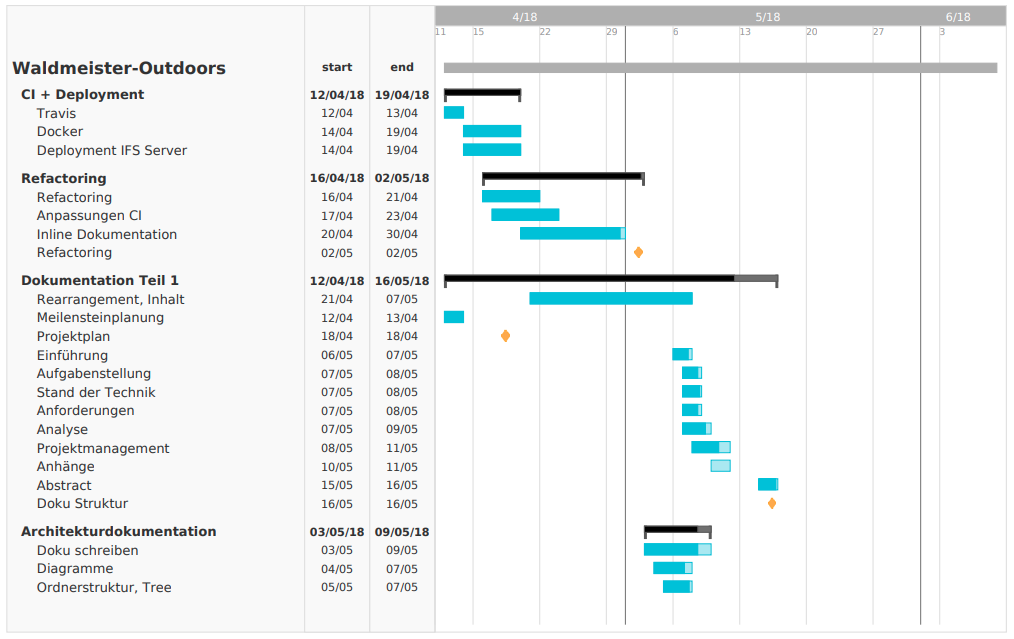
\includegraphics[width=1\textwidth]{gantt1}
    \caption{Gantt Diagramm Teil 1}
    \label{fig:gantt1}
\end{figure}

\begin{figure}[H]
    \centering
    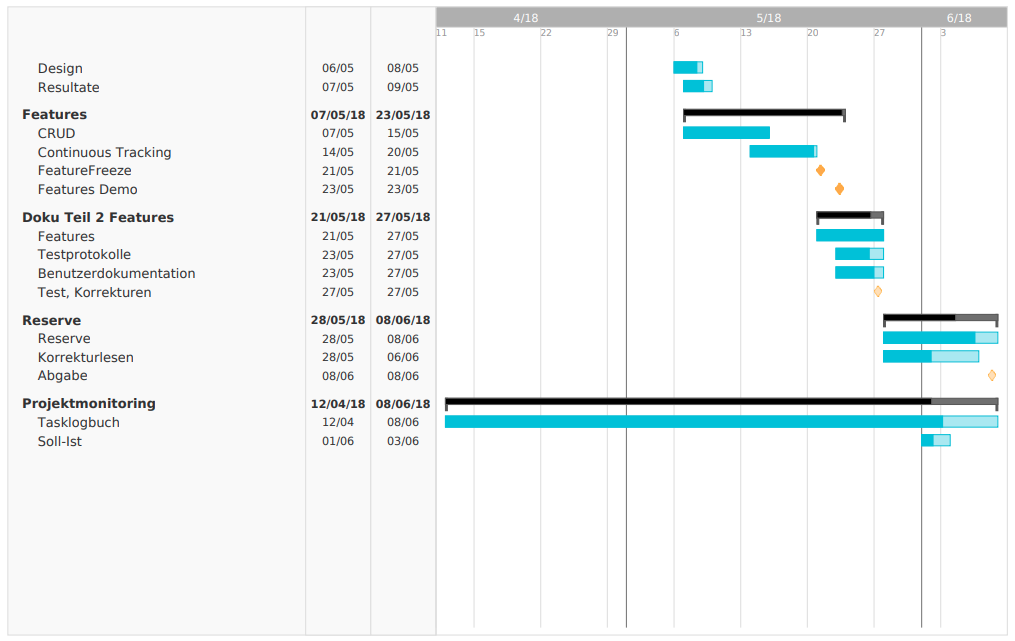
\includegraphics[width=1\textwidth]{gantt2}
    \caption{Gantt Diagramm Teil 2}
    \label{fig:gantt2}
\end{figure}
\pagebreak

\subsection{Entwicklungswerkzeuge}
Als Texteditor, bzw. IDE wurde Sublime eingesetzt welches Linter f\"ur JavaScript und Python unterst\"utzt. Sublime ist open-source und st\"utzt sich auf viele Pakete, welche im integrierten Package-Manager heruntergeladen und konfiguriert werden k\"onnen. $\newline$
GitHub wurde Verwendet um eine Versionierung des Programmcodes zu erm\"oglichen. Issues werden auf GitHub erstellt.

\subsection{Git, GitHub}
Git wurde zur Versionenkontrolle des Projekts verwendet. Versionenkontrolle erlaubt es, verschiedene Versionen eines Projekts zu haben und zeigt die \"Anderungen, welche im Code \"uber Zeit gemacht wurden. Git erlaubt es auch, \"Anderungen r\"uckg\"angig zu machen und ist vorallem bei gr\"osseren Projekten von unerl\"asslichem Nutzen. Bei Git, anstelle eines zentralen Servers, welcher die aktuellste Version hostet, haben bei Git alle beteiligten Entwickler die gesamte "version history" des Projekts auf all Ihren Ger\"aten, statt nur die aktuellste Version, welche sie Lokal gespeichert haben. User haben jederzeit Zugriff auf alle Versionen aller Dateien im Git-Repository. Mehrere Entwickler k\"onnen gleichzeitig an einem Projekt arbeiten, ohne sich gegenseitig zu st\"oren, und haben keine Angst, die von einem Kollegen vorgenommenen \"Anderungen zu verlieren. In Git sind die M\"oglichkeiten der Zusammenarbeit unbegrenzt. Git ist gratis und open-source. $\newline$
Github ist ein Remote Server f\"ur Git Projekte, welcher gleichzeitig ein Community Hub f\"ur Entwickler ist. Auf Github k\"onnen Repositories mit einem grafischen web Interface bearbeitet werden, und Entwickler k\"onnen sich \"uber Projekte informieren und teilnehmen.

\begin{figure}[H]
    \centering
    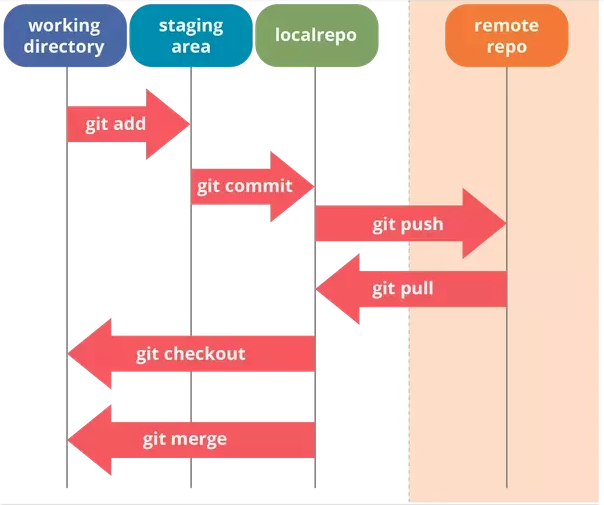
\includegraphics[width=0.6\textwidth]{github}
    \caption{Git und Github Operationen}
    \label{fig:mesh1}
\end{figure}

\subsection{Projektboards}
Mit den Projektboards auf GitHub k\"onnen Softwareprojekte organisiert und Aspekte priorisiert werden. Projektboards k\"onnen f\"ur spezifische Funktionen, umfassende Roadmaps oder sogar Release-Checklisten erstellt werden. Projektboards bestehen aus Themen, Pull-Requests und Notizen, die in Spalten als Karten kategorisiert werden, zum Beispiel "To Do", "In Progress", "Ready to Review" und "Done". Notizen und Issues k\"onnen innerhalb einer Karte dargestellt werden und wechseln w\"ahrend ihrer Entwicklung die Karten / Spalten bis sie in der Karte "Done" bleiben. Dies kann sogar automatisiert werden. \cite{githubauto} $\newline$ 
Notizen und Issues k\"onnen Bugs, Features, Aufgabenerinnerungen oder Tasks welche in der Planungsphase anfallen, m\"ussen daher nicht direkt mit der Codebase zu tun haben. Neben Repository-weiten Projektboards gibt es auch Organisations-weite Projektboards, welche Probleme und Anfragen von allen Repositories beinhalten, die zu einer Organisation geh\"ort.

\subsection{Issues}
W\"ahrend dem Projekt und insbesondere w\"ahrend der Projektplanungsphase werden Issues erfasst, welche geplante Schritte, Funktionen oder Arbeitsschritte beschreiben. Issues sind in die Kategorien "To Do", "In Progress", "Ready to Review" und "Done and Reviewed" unterteilt. Issues k\"onnen w\"ahrend der Entwicklung mehrmals Ihre Kategorie wechseln, zum Beispiel bei einem Review wieder in die Kategorie "To Do" eingeteilt werden. Issues haben einen "Label", welche sie einer Gruppierung wie "Bug", "Must Have" oder "Dokumentation" zuordnen. $\newline$
Issues sind auch einem Meilenstein zugeordnet, damit in der Projekt\"ubersicht ersichtlich ist, welche Meilensteine abgeschlossen oder "overdue" sind.

\subsection{Releases}
Als Release wird das Deployment der Webapp auf den Produktions Server bezeichnet. Grunds\"atzlich wird die Webapp auf einem Lokalen Testserver entwickelt und getestet. Bei einem Release wird die Lauff\"ahige Webapp auf das Livesystem portiert und \"offentlichen Usern zug\"anglich gemacht. 


\subsection{Zeitplan}
Eine grobe Planung wurde Anfangs April festgehalten. Es wurde eine Meilensteinplanung sowie eine Aufwandsch\"atzung und ein Projektplan als Gantt-Diagramm festgehalten. Issues wurden am Anfang des Projekt bereits einige definiert, wurden jedoch laufend im GitHub Projektboard auf dem neusten Stand gehalten.


\subsection{Risiken}

\begin{table}[H]
\centering
\begin{tabular}{|l|l|l|l|l|}
\hline
\multicolumn{5}{|l|}{R01: Mangelnde Erfahrung mit VueJS}                                                                                                                                                                                                                                                                                         \\ \hline
Beschreibung                     & \multicolumn{4}{l|}{Wirkt sich negativ auf Design und Programmcode aus.}                                                                                                                                                                                                                                      \\ \hline
Schadenspotential                & \multicolumn{4}{l|}{30h}                                                                                                                                                                                                                                                                                      \\ \hline
Eintrittswahrscheindlichkeit     & \multicolumn{4}{l|}{80\%}                                                                                                                                                                                                                                                                                     \\ \hline
Auswirkung                       & \multicolumn{4}{l|}{\begin{tabular}[c]{@{}l@{}}VueJS wird als Frontend Framework eingesetzt. Es Umfasst die \\ ganze visuelle Darstellung der Webapplikation und ist daf\"ur \\ zust\"andig, dass die Navigation und Aufruf der API Requests \\ korrekt ausgef\"uhrt wird.\end{tabular}}                            \\ \hline
Vorbeugung                       & \multicolumn{4}{l|}{\begin{tabular}[c]{@{}l@{}}Vue kann an vielen Orten eingesetzt werden um visuelle oder \\ funktionelle Anforderungen zu \"ubernehmen. Mittels JavaScript \\ Libraries wie Vuetify kann bei der visuellen Darstellung auf \\ Vorgefertigte Komponenten zur\"uckgegriffen werden.\end{tabular}} \\ \hline
\end{tabular}
\caption{VueJS Risiken}
\label{my-label}
\end{table}


\begin{table}[H]
\centering
\begin{tabular}{|l|l|l|l|l|}
\hline
\multicolumn{5}{|l|}{R02: Fehlende Erfahrung mit Python / Django}                                                                                                                                                                                                                                                                                                                                                                                                                                     \\ \hline
Beschreibung                      & \multicolumn{4}{l|}{Wirkt sich negativ auf Performance und Security aus}                                                                                                                                                                                                                                                                                                                                                                                          \\ \hline
Schadenspotential                 & \multicolumn{4}{l|}{20h}                                                                                                                                                                                                                                                                                                                                                                                                                                          \\ \hline
Eintrittswahrscheindlichkeit      & \multicolumn{4}{l|}{80\%}                                                                                                                                                                                                                                                                                                                                                                                                                                         \\ \hline
Auswirkung                        & \multicolumn{4}{l|}{\begin{tabular}[c]{@{}l@{}}Das Django-Backend basiert auf Python. Das Frontend fragt\\ Informationen zu Login und Benutzerfl\"achen beim Backend\\ ab. Rest-Schnittstellen und Serializer werden vom Backend\\ bereitgestellt und m\"ussen korrekt funktionieren, damit keine \\ Sicherheitsl\"ucken entstehen. Bei einer falschen Konfiguration\\ des Backends k\"onnen auch geschwindigkeitsrelevante Probleme\\ beim Frontend auftreten.\end{tabular}} \\ \hline
Vorbeugung                        & \multicolumn{4}{l|}{\begin{tabular}[c]{@{}l@{}}Python Pakete verwenden, welche die Authorisierung\\ von Usern korrekt ausf\"uhren und die geschwindigkeitsrelevante\\ API Abfragen in realen Umgebungen testen und ggf. \\ verbessern. Auf Tutorial und Guides setzen um das API\\ zu erstellen.\end{tabular}}                                                                                                                                                         \\ \hline
\end{tabular}
\caption{Django / Python Risiko}
\label{my-label}
\end{table}


\begin{table}[H]
\centering
\begin{tabular}{|l|l|l|l|l|}
\hline
\multicolumn{5}{|l|}{R03: Fehlende Erfahrung mit Leaflet \& Leaflet Editable}                                                                                                                                                                                                                                                                                                                                                                              \\ \hline
Beschreibung                         & \multicolumn{4}{l|}{Wirkt sich negativ auf Usability und Funktionalit\"at aus}                                                                                                                                                                                                                                                                                                                                        \\ \hline
Schadenspotential                    & \multicolumn{4}{l|}{30h}                                                                                                                                                                                                                                                                                                                                                                                            \\ \hline
Eintrittswahrscheindlichkeit         & \multicolumn{4}{l|}{70\%}                                                                                                                                                                                                                                                                                                                                                                                           \\ \hline
Auswirkung                           & \multicolumn{4}{l|}{\begin{tabular}[c]{@{}l@{}}Ein Grossteil der User-Interaktion findet beim Frontend\\ auf dem Map Objekt statt. Das Erstellen, bzw. Bearbeiten\\ von Benutzerfl\"achen wird von Leaflet Editable bereitgestellt,\\ muss jedoch korrekt implementiert werden, damit die\\ Zusammenarbeit mit dem Backend korrekt funktioniert.\end{tabular}}                                                        \\ \hline
Vorbeugung                           & \multicolumn{4}{l|}{\begin{tabular}[c]{@{}l@{}}Leaflet Beispiele verwenden um Benutzerfl\"achen und \\ GeoJSON Layer korrekt darzustellen. \\ Leaflet-editable Code korrekt implementieren damit beim \\ Aufruf von API Abfragen keine Fehler passieren.\\ Bestehende Features testen bevor neue Features \\ implementiert werden. Codebase oft Refaktorisieren.\\ Zusammenarbeit mit VueJS \"uberpr\"ufen.\end{tabular}} \\ \hline
\end{tabular}
\caption{Risiko Leaflet & Leaflet-editable}
\label{my-label}
\end{table}

\begin{table}[H]
\centering
\begin{tabular}{|l|l|l|l|l|}
\hline
\multicolumn{5}{|l|}{R04: Leistung von mobilen Ger\"aten schw\"acher}                                                                                                                                                                                                                                                                                                               \\ \hline
Beschreibung                      & \multicolumn{4}{l|}{Wirkt sich negativ auf Usability aus}                                                                                                                                                                                                                                                                                   \\ \hline
Schadenspotential                 & \multicolumn{4}{l|}{15h}                                                                                                                                                                                                                                                                                                                    \\ \hline
Eintrittswahrscheindlichkeit      & \multicolumn{4}{l|}{80\%}                                                                                                                                                                                                                                                                                                                   \\ \hline
Auswirkung                        & \multicolumn{4}{l|}{\begin{tabular}[c]{@{}l@{}}Mobile Ger\"ate haben Schwierigkeiten viele Objekte\\ auf der Leaflet Map darzustellen. Waldstandortsfl\"achen\\ des Vegetationslayers k\"onnen das Ger\"at \"uberfordern,\\ auch wenn die Darstellung und Usability bei\\ Desktopger\"aten gew\"ahrleistet ist.\end{tabular}}                             \\ \hline
Vorbeugung                        & \multicolumn{4}{l|}{\begin{tabular}[c]{@{}l@{}}Anzahl an Objekten, welche auf der Leaflet Map \\ dargestellt werden reduzieren. Fl\"achen welche nicht\\ im Kartenausschnitt sichtbar sind nicht laden um\\ das Mobile Ger\"at nicht zu \"uberfordern.\\ Komplexit\"at (Genauigkeit) der Polygone des \\ Vegetationslayers reduzieren\end{tabular}} \\ \hline
\end{tabular}
\caption{Risiko Leistung Mobile Ger\"ate}
\label{my-label}
\end{table}

\subsection{Zusammenfassung Risiken}
Aus den Risiken gehen Schadenspotentiale hervor, welche in der Projektplanung ber\"ucksichtigt werden m\"ussen. Da die Risiken aus Technologien hervorgehen, ist vorhersehbar in welchem Projektabschnitt sie auftreten k\"onnten. Neben einer Reservezeit werden diese Risiken vorallem dazu verwendet den jeweiligen Meilensteinen mehr Zeit zuzurechnen. $\newline$
Risiko 1: $\newline$
30h * 0.8 = 24h$\newline$
$\newline$
Risiko 2:$\newline$
20h * 0.8 = 16h$\newline$
$\newline$
Risiko 3:$\newline$
30h * 0.7 = 21h$\newline$
$\newline$
Risiko 4:$\newline$
15h * 0.8 = 12h$\newline$
$\newline$
Total: 73 Stunden$\newline$
$\newline$
Um diesen Risiken vorzubeugen wurde vor den Sprints abgekl\"art und getestet wie relevant die Risiken bei der Implementation sein werden. Falls die Risiken bei der Abkl\"arung auftauchen wurden die Sprints in kleinere Teile zerlegt bzw. mehr Zeit eingeplant.


\section{Projektmonitoring}
\subsection{Soll-Ist-Zeitvergleich}
Die 180 geplanten Stunden seit 11.4. wurden auf 9 Wochen aufgeteilt, damit die Abgabe am 8.6. erfolgen kann. Dadurch ergibt sich einen durchschnittlichen Aufwand von 20 Stunden pro Woche. Tats\"achlich gearbeitet wurden 238 Stunden (Durchschnittlich 26 Stunden pro Woche). Mehr Zeit kamen vor allem beim Deployment und der Entwicklung der Features auf. Die Risiken wurden korrekt abgesch\"atzt, wobei am meisten zus\"atzliche Zeit bei Django / Python und Leaflet Editable aufgewendet wurde.
\subsection{Code Statistics}
Das Projekt umfasst 11954 Lines of Code. Analysiert wurde das lokale Projektfolder, ohne Node Modules, Dokumentation und statischen Files. Es wurde das Node Package Cloc verwendet um diese Codestatistik zu generieren. (Stand 6.6.2018)

\section{Softwaredokumentation}
\subsection{Installation}
Um die App zu verwenden, sollte die Anleitung auf GitHub (Readme) verwendet werden, oder die .yml config Datei, um das Projekt auf einer Linux Machine zu builden. $\newline$
$\newline$
Github Repo klonen $\newline$ $\newline$
"npm install" $\newline$ $\newline$
"pip install -r requirements.txt" $\newline$ $\newline$
"npm start" im client folder startet den Vue-Server $\newline$ $\newline$
"python manage.py runserver" (als separates Window oder Tab) im root Folder startet den Django Server $\newline$ $\newline$
Damit Django die PostgreSQL Datenbank verwenden kann, m\"ussen die Werte in der settings.py angepasst werden, oder eine Datenbank mit dem Namen dschwaldmeister, user Postgres und Port 5432 erstellt werden. Von PostgreSQL soll auch die Extension postgis erzeugt werden. $\newline$
Mit "manage.py migrate" kann die Datenbank auf den neusten Stand gebracht werden, damit sie verwendet werden kann. $\newline$
Die App kann im Browser unter der angezeigten Adresse des Vue-Servers aufgerufen werden. $\newline$
$\newline$
Alternativ kann das Projekt mit dem Befehl "docker-compose build" in Dockercontainern gebuildet und mit "docker-compose up" ausgef\"uhrt werden. $\newline$
Das Projekt ist im Internet unter \href{https://waldmeistermap.sifs0003.infs.ch/}{waldmeister-outdoors} deployt.

\subsection{Tutorial, Handbuch}
Registrierung: $\newline$
Um einen neuen Benutzer zu registrieren, muss ein bereits eingeloggter User sich ausloggen. Danach kann mit der Schaltfl\"ache "Register" ein neuer Account erstellt werden. Username und Passwort werden ben\"otigt, Email ist optional und kann leer gelassen werden.
$\newline$
$\newline$
Fl\"ache Erstellen:$\newline$
Ein eingeloggter User hat die M\"oglichkeit eine Neue Benutzerfl\"ache zu erstellen. Um dies zu tun, muss er auf die Schaltfl\"ache "Add" auf der linken Seite, unterhalb der Zoom Buttons klicken. Im Editiermodus kann er durch Klicks auf die Map neue Eckpunkte zu einem Polygon hinzuf\"ugen. Er kann die Fl\"ache schliessen, in dem er auf den ersten erstellten Eckpunkt klickt. Es \"offnet sich eine Dialogbox, in welchem der User der erstellten Fl\"ache einen Namen geben kann, welcher auf der Map erscheint. In dieser Dialogbox kann der User auch entscheiden, ob die Fl\"ache \"offentlich (f\"ur alle sichtbar) oder privat dargestellt werden soll (nur f\"ur den User sichtbar, welcher die Fl\"ache erstellt hat).
$\newline$
$\newline$
Fl\"ache Bearbeiten:$\newline$
Um eine bereits erstellte Fl\"ache zu bearbeiten und zu ver\"andern muss die zu \"andernde Fl\"ache angew\"ahlt werden, w\"ahrend der User, welcher die Fl\"ache erstellt hat, eingeloggt ist. Nur der User, der die Benutzerfl\"ache erstellt hat, kann diese Ver\"andern oder Updaten. Im Bearbeitungsmodus kann der User die Eckpunkte des Polygons beliebig verschieben. Durch einen Klick auf die Schaltfl\"ache "Upd" (Update), \"offnet sich die Dialogbox, um der Benutzerfl\"ache einen neuen Namen zu geben, oder Ihren Zustand von \"offentlich oder privat zu wechseln.
$\newline$
$\newline$
Fl\"ache L\"oschen: $\newline$
Im eingeloggten Zustand auf eine mit diesem User erstellte Benutzerfl\"ache klicken. Durch Klick auf den Button "Del" am linken Rand der Map wird die ausgew\"ahlte Fl\"ache gel\"oscht.

\subsection{Projektrelevante Links}
Projekt Wiki$\newline$
\href{https://wiki.hsr.ch/StefanKeller/wiki.cgi?PA2_FS18_Schmider_Aufgabenstellung_2 }{Projekt Wiki HSR}$\newline$$\newline$
Github und Github Projekt $\newline$
\href{https://github.com/dschmide/Waldmeister}{GitHub} $\newline$
\href{https://github.com/dschmide/Waldmeister/projects/1}{Projektseite} $\newline$ $\newline$
Gis-Browser Kanton Z\"urich $\newline$
\href{https://maps.zh.ch?topic=WaldVKZH&scale=18634&x=2706590.13&y=1251180.39&srid=2056}{Gis Browser}$\newline$ $\newline$
Giswiki Koordinatensystem$\newline$
\href{https://giswiki.hsr.ch/Koordinatensystem}{Koordinatensystem} $\newline$ $\newline$
Native Waldmeister App f\"ur Android und iOS Ger\"ate $\newline$
\href{https://itunes.apple.com/bn/app/waldmeister/id825753160?mt=8}{Appstore} $\newline$
\href{https://play.google.com/store/apps/details?id=bgu\_schmider.waldmeister}{Playstore} $\newline







